\documentclass{article}
%Usepackages
\usepackage{adjustbox, amsmath, amssymb, amsthm, blindtext, bm, bbm, dblfloatfix, esint, fancyhdr, float, graphicx, letltxmacro, marginnote, mathtools, subcaption, xcolor, titlesec, esint}
\usepackage{amssymb}
\usepackage[font={small, it}]{caption}
\usepackage{amsmath}
\usepackage{floatrow}
\usepackage{times}
\usepackage{ stmaryrd }
\usepackage{amsthm}
\usepackage{xcolor}
\usepackage{soul}
\usepackage{mathrsfs}
\usepackage[colorlinks = true,
            linkcolor = black,
            urlcolor  = blue,
            citecolor = black,
            anchorcolor = blue]{hyperref}
% \usepackage[mathscr]{euscript}
\usepackage{mathrsfs}
\usepackage{wasysym}
%\usepackage{pxfonts}
\usepackage[letterpaper, portrait, margin=1in]{geometry}
\usepackage{graphicx}
\usepackage{tikz}
\usepackage{tikz-3dplot}
\usepackage{pgfplots}
\usetikzlibrary{decorations.pathmorphing,patterns}
\usepackage{lipsum}
\usepackage{float}
\usepackage{subcaption}
\usepackage[object=vectorian]{pgfornament}
\usepackage{mwe}
\usepackage{bigints}
\usepackage{csquotes}
\usepackage{titlesec}
\usepackage{halloweenmath}
\setcounter{secnumdepth}{4}
\titleformat{\paragraph}
{\normalfont\normalsize\bfseries}{\theparagraph}{1em}{}
\titlespacing*{\paragraph}
{0pt}{3.25ex plus 1ex minus .2ex}{1.5ex plus .2ex}
\usepackage{mathtools}
\usepackage{pgfplots}
\pgfplotsset{compat=1.15}
\usepackage{lastpage}
\usepackage{enumitem}
\usepackage{tensor}
\usepackage{mathtools}

% This is for the header:
% https://tex.stackexchange.com/questions/75168/get-current-section-name-without-label
\usepackage{nameref}
\makeatletter
\newcommand*{\currentname}{\@currentlabelname}
\makeatother

\usepackage{fancyhdr} 
    \pagestyle{fancy}
    \fancyhf{}
    \fancyhead[R]{ Page \thepage \  of \pageref{LastPage}}
    \fancyhead[L]{\currentname}
\usepackage{setspace}
\usepackage{tikz}
\usetikzlibrary{hobby}

\usepackage{pst-node}
\usepackage{tikz-cd}
\usepackage[most]{tcolorbox}

% \makeatletter
% \renewcommand\@endtheorem{\vvv@endmarker\endtrivlist\@endpefalse}
% \newcommand\vvv@endmarker{%
%   {\unskip\nobreak\hfil\penalty50
%   \hskip2em\vadjust{}\nobreak\hfil\openbox
%   \parfillskip=0pt \finalhyphendemerits=0 \par
%   \penalty 10000 \parskip=0pt\noindent}\ignorespaces}
% \makeatother

\theoremstyle{definition}

% https://tex.stackexchange.com/questions/616586/how-to-make-a-tcolorbox-with-only-a-left-side-rule


\newtheorem{thm}{Theorem}[section]
\newtheorem{defn}[thm]{Definition}
\newtheorem{exmp}[thm]{Example}
\newtheorem{lem}[thm]{Lemma}
\newtheorem{conjecture}[thm]{Conjecture}
\newtheorem{exercise}[thm]{Exercise}
\newtheorem{fact}[thm]{Fact}
\newtheorem{claim}[thm]{Claim}
\newtheorem{cor}[thm]{Corollary}
\newtheorem{summary}[thm]{Summary}

\newtheorem{idea}[thm]{Idea}
\newtheorem{application}[thm]{Application}
\newtheorem{rmk}[thm]{Remark}

\newtheorem{prop}[thm]{Proposition}
\newtheorem{ques}[thm]{Question}
\newtheorem{observation}[thm]{Observation}

\newtcolorbox{cbox}[1][]{
            breakable,
            boxrule=0pt,
            frame hidden,
            sharp corners,
            enhanced,
            borderline west={2pt}{0pt}{#1},
            colback=#1!5!white}

% \newenvironment{cthm}[3]
%     {\begin{cbox}[#2]
%     \color{#2}
%     \begin{#3}[#1]
%     \color{black}
%     }
%     {
%     \end{#3} 
%     \end{cbox}
%     }

% \newenvironment{theorem}[1][]
% {\begin{cthm}{#1}{orange}{thm}}
% {\end{cthm}}

\newenvironment{theorem}[1][]
    {\begin{cbox}[blue]
    \color{blue}
    \begin{thm}[#1]
    \color{black}
    }
    {
    \end{thm} 
    \end{cbox}
    }

\newenvironment{corollary}[1][]
    {\begin{cbox}[orange]
    \color{orange}
    \begin{cor}[#1]
    \color{black}
    }
    {
    \end{cor} 
    \end{cbox}
    }

\newenvironment{lemma}[1][]
    {\begin{cbox}[orange]
    \color{orange}
    \begin{lem}[#1]
    \color{black}
    }
    {
    \end{lem} 
    \end{cbox}
    }

\newenvironment{proposition}[1][]
    {\begin{cbox}[orange]
    \color{orange}
    \begin{prop}[#1]
    \color{black}
    }
    {
    \end{prop} 
    \end{cbox}
    }

\newenvironment{definition}[1][]
    {\begin{cbox}[red]
    \color{red}
    \begin{defn}[#1]
    \color{black}
    }
    {
    \end{defn} 
    \end{cbox}
    }

\newenvironment{example}[1][]
    {\begin{cbox}[violet]
    \color{violet}
    \begin{exmp}[#1] \color{black}
    }
    {
    \end{exmp} 
    \end{cbox}
    }

\newenvironment{question}[1][]
    {\begin{cbox}[black]
    \begin{ques}[#1]
    }
    {
    \end{ques} 
    \end{cbox}
    }

\newenvironment{remark}[1][]
    {\begin{cbox}[black]
    \begin{rmk}[#1]
    }
    {
    \end{rmk} 
    \end{cbox}
    }



\newenvironment{solution}
  {\renewcommand\qedsymbol{$\blacksquare$}\begin{proof}[Solution]}
  {\end{proof}}
\newenvironment{answer}
  {\begin{proof}[Answer]}
  {\end{proof}}
  
% \newenvironment{example}
%   {\pushQED{\qed}\renewcommand{\qedsymbol}{$\triangle$}\examplex}
%   {\popQED\endexamplex}


%%%%%%%%%%%%%%%%%%%%%%%%%%%%%

%Custom Commands
    \renewcommand\qedsymbol{$\blacksquare$}
    \newcommand{\Pcal}{\mathcal{P}}
    \newcommand{\ve}{\varepsilon}
    \newcommand{\Ocal}{\mathcal{O}}
    \newcommand{\Asf}{\textsf{A}}
    \newcommand{\al}{\alpha}
    \newcommand{\be}{\beta}
    \newcommand{\Nbb}{\mathbb{N}}
    \newcommand{\Si}{\Sigma}
    \newcommand{\Hbb}{\mathbb{H}}
    \DeclareMathOperator{\diag}{diag}
    \newcommand{\De}{\Delta}
    \newcommand{\Xcal}{\mathcal{X}}
    \newcommand{\si}{\sigma}
    \newcommand{\Ga}{\Gamma}
    \newcommand{\Cscr}{\mathscr{C}}
    \newcommand{\1}{\mathbf{1}}
    \newcommand{\Dcal}{\mathcal{D}}
    \newcommand{\Iscr}{\mathscr{I}}
    \newcommand{\Pbb}{\mathbb{P}}
    \newcommand{\B}{\mathbb{B}}
    \newcommand{\Dscr}{\mathscr{D}}
    \newcommand{\Nfrak}{\mathfrak{N}}
    \newcommand{\Efrak}{\mathfrak{E}}
    \DeclareMathOperator{\charp}{charpoly}
    \newcommand{\Csf}{\mathsf{C}}
    \newcommand{\rfrak}{\mathfrak{r}}
    \newcommand{\Sbb}{\mathbb{S}}
    \newcommand{\La}{\Lambda}
    \newcommand{\de}{\delta}
    \DeclareMathOperator{\inte}{int}
    \DeclareMathOperator{\ord}{ord}
    \newcommand{\set}{\mathsf{set}}
    \newcommand{\Bscr}{\mathscr{B}}
    \newcommand{\Zscr}{\mathscr{Z}}
    \newcommand{\ab}{\mathrm{ab}}
    \newcommand{\Xscr}{\mathscr{X}}
    \newcommand{\Escr}{\mathscr{E}}
    \newcommand{\Gscr}{\mathscr{G}}
    \DeclareMathOperator{\Sym}{Sym}
    \newcommand{\om}{\omega}
    \newcommand{\gfrak}{\mathfrak{g}}
    \newcommand{\hfrak}{\mathfrak{h}}
    \newcommand{\kfrak}{\mathfrak{k}}
    \newcommand{\Grp}{\mathsf{Grp}}
    \newcommand{\Ab}{\mathsf{Ab}}
    \newcommand{\xbar}{\bar{x}}
    \newcommand{\abar}{\bar{a}}
    \newcommand{\ybar}{\bar{y}}
    \DeclareMathOperator{\coker}{coker}
    \newcommand{\Modsf}{\mathsf{Mod}}
    \newcommand{\op}{\mathrm{op}}
    \newcommand{\Ring}{\mathsf{Ring}}
    \newcommand{\modsf}{\mathsf{mod}}
    \DeclareMathOperator{\Alt}{Alt}
    \newcommand{\Om}{\Omega}
    \newcommand{\ze}{\zeta}
    \newcommand{\Fcal}{\mathcal{F}}
    \newcommand{\Oscr}{\mathscr{O}}
    \newcommand{\gl}{\mathfrak{gl}}
    \DeclareMathOperator{\Lie}{Lie}
    \DeclareMathOperator{\GL}{GL}
    \DeclareMathOperator{\SL}{SL}
    \DeclareMathOperator{\Vol}{Vol}
    \DeclareMathOperator{\Disc}{Disc}
    \DeclareMathOperator{\SO}{SO}
    \newcommand{\Xfrak}{\mathfrak{X}}
    \DeclareMathOperator{\id}{id}
    \DeclareMathOperator{\Int}{Int}
    \DeclareMathOperator{\End}{End}
    \DeclareMathOperator{\Aut}{Aut}
    \DeclareMathOperator{\stab}{stab}
    \DeclareMathOperator{\orb}{orb}
    \DeclareMathOperator{\grad}{grad}
    \DeclareMathOperator{\curl}{curl}
    \newcommand{\vp}{\varphi}
    \newcommand{\vt}{\vartheta}
    \DeclareMathOperator{\Gal}{Gal}
    \DeclareMathOperator{\rank}{rank}
    \DeclareMathOperator{\col}{col}
    \DeclareMathOperator{\Tame}{Tame}  
    \newcommand{\Yscr}{\mathscr{Y}}
    \newcommand{\Fbb}{\mathbb{F}}
    \newcommand{\Hcal}{\mathcal{H}}
    \newcommand{\arctanh}{\text{arctanh}}
    \newcommand{\pa}{\partial}
    \newcommand{\del}{\boldsymbol{\nabla}}
    \newcommand{\na}{\nabla}
    \newcommand{\Ycal}{\mathcal{Y}}
    \DeclareMathOperator{\spn}{span}
    \DeclareMathOperator{\Inn}{Inn}
    \DeclareMathOperator{\chara}{char}
    \newcommand{\lap}{\nabla^2}
    \newcommand{\Pfrak}{\mathfrak{P}}
    \newcommand{\mfrak}{\mathfrak{m}}
    \newcommand{\Fvec}{\mathbf{F}}
    \newcommand{\Mcal}{\mathcal{M}}
    \newcommand{\ellvec}{\boldsymbol{\ell}}
    \newcommand{\rvec}{\mathbf{r}}
    \DeclareMathOperator{\supp}{supp}
    \newcommand{\Abb}{\mathbb{A}}
    \newcommand{\svec}{\mathbf{s}}
    \newcommand{\VECT}{\mathsf{VECT}}
    \newcommand{\fs}{\vec{\sigma}}
    \newcommand{\bs}{\cev{\sigma}}
    \newcommand{\uvec}{\mathbf{u}}
    \newcommand{\iunit}{\boldsymbol{\hat{\i}}}
    \newcommand{\junit}{\boldsymbol{\hat{\j}}}
    \newcommand{\xunit}{\mathbf{\hat{x}}}
    \newcommand{\Char}{\text{char}}
    \newcommand{\kunit}{\mathbf{\hat{k}}}
    \newcommand{\theunit}{\boldsymbol{\hat{\theta}}}
    \newcommand{\pvec}{\mathbf{p}}
    \newcommand{\qvec}{\mathbf{q}}
    \newcommand{\Qcal}{\mathcal{Q}}
    \newcommand{\yvec}{\mathbf{y}}
    \newcommand{\xvec}{\mathbf{x}}
    \newcommand{\wvec}{\mathbf{w}}
    \newcommand{\bvec}{\mathbf{b}}
    \newcommand{\Ucal}{\mathcal{U}}
    \newcommand{\Ncal}{\mathcal{N}}
    \newcommand{\Scal}{\mathcal{S}}
    \newcommand{\Nscr}{\mathscr{N}}
    \newcommand{\da}{\dagger}
    \newcommand{\CT}{\mathrm{H}}
    \newcommand{\Sscr}{\mathscr{S}}
    \DeclareMathOperator{\lcm}{lcm}
    \newcommand{\evec}{\mathbf{e}}
    \newcommand{\Kscr}{\mathscr{K}}
    \newcommand{\ebold}{\boldsymbol{e}}
    \newcommand{\zvec}{\mathbf{z}}
    \newcommand{\vvec}{\mathbf{v}}
    \newcommand{\Tscr}{\mathscr{T}}
    \newcommand{\avec}{\mathbf{a}}
    \newcommand{\Avec}{\mathbf{A}}
    \newcommand{\Ivec}{\mathbf{I}}
    \newcommand{\ivec}{\mathbf{i}}
    \newcommand{\jvec}{\mathbf{j}}
    \newcommand{\kvec}{\mathbf{k}}
    \newcommand{\of}{\mathfrak{o}}
    \DeclareMathOperator{\Ot}{O}
    \DeclareMathOperator{\Sy}{S}
    \newcommand{\slf}{\mathfrak{sl}}
    \newcommand{\muvec}{\boldsymbol{\mu}}
    \newcommand{\Bvec}{\mathbf{B}}
    \newcommand{\Cvec}{\mathbf{C}}
    \newcommand{\eunit}{\mathbf{\hat{e}}}
    \newcommand{\vpunit}{\boldsymbol{\hat{\varphi}}}
    \newcommand{\zero}{\boldsymbol{0}}
    \newcommand{\tauvec}{\boldsymbol{\tau}}
    \newcommand{\runit}{\mathbf{\hat{r}}}
    \newcommand{\U}{\mathcal{U}}
    \newcommand{\Zbb}{\mathbb{Z}}
    \newcommand{\Dbb}{\mathbb{D}}
    \newcommand{\Bsf}{\mathsf{B}}
    \DeclareMathOperator{\G}{G}
    \newcommand{\gmat}{\textsf{g}}
    \newcommand{\Ccal}{\mathcal{C}}
    \newcommand{\SM}{\mathsf{SM}}
    \newcommand{\VB}{\mathsf{VB}}
    \newcommand{\Dsf}{\mathsf{D}}
    \newcommand{\Fscr}{\mathscr{F}}
    \DeclareMathOperator{\Map}{Map}
    \DeclareMathOperator{\Frob}{Frob}
    \newcommand{\Imat}{\textsf{I}}
    \newcommand{\Rmat}{\textsf{R}}
    \DeclareMathOperator{\Frac}{Frac}
    \DeclareMathOperator{\Spec}{Spec}
    \DeclareMathOperator{\Emb}{Emb}
    \newcommand{\Kcal}{\mathcal{K}}
    \newcommand{\Wcal}{\mathcal{W}}
    \newcommand{\Lcal}{\mathcal{L}}
    \newcommand{\Tcal}{\mathcal{T}}
    \newcommand{\Ecal}{\mathcal{E}}
    \DeclareMathOperator{\im}{im}
    \newcommand{\Qbb}{\mathbb{Q}}
    \newcommand{\ga}{\gamma}
    \newcommand{\la}{\lambda}
    \newcommand{\RomanNumeralCaps}[1]
        {\MakeUppercase{\romannumeral #1}} 
    \newcommand{\dif}{\text{d}}
    \newcommand{\Rbb}{\mathbb{R}}
    \newcommand{\Tbb}{\mathbb{T}}
    \DeclareMathOperator{\Hom}{Hom}
    \DeclareMathOperator{\conv}{conv}
    \newcommand{\Vcat}{\mathsf{V}}
    \newcommand{\Gr}{\text{Gr}}
    \newcommand{\Bcal}{\mathcal{B}}
    \newcommand{\Acal}{\mathcal{A}}
    \newcommand{\pfrak}{\mathfrak{p}}
    \newcommand{\qfrak}{\mathfrak{q}}
    \newcommand{\Evec}{\mathbf{E}}
    \newcommand{\omvec}{\boldsymbol{\omega}}
    \newcommand{\alvec}{\boldsymbol{\alpha}}
    \newcommand{\gvec}{\mathbf{g}}
    \newcommand{\afrak}{\mathfrak{a}}
    \newcommand{\bfrak}{\mathfrak{b}}
    \newcommand{\Cbb}{\mathbb{C}}
    \newcommand{\gavec}{\boldsymbol{\gamma}}
    \newcommand{\Tvec}{\mathbf{T}}
    \newcommand{\Vscr}{\mathscr{V}}
    \newcommand{\Ascr}{\mathscr{A}}
    \newcommand{\Uscr}{\mathscr{U}}
    \newcommand{\Sfrak}{\mathfrak{S}}
    \DeclareMathOperator{\sgn}{sgn}
    \DeclareMathOperator{\vol}{vol}
    \newcommand{\Pscr}{\mathscr{P}}
    \newcommand{\Wscr}{\mathscr{W}}
    \newcommand{\bcdot}{\boldsymbol{\cdot}}
    \DeclareMathOperator{\tr}{tr}
    
    \newcommand{\sectionline}{
        \noindent
        \begin{center}
        {
        {{
        {\begin{tikzpicture}
        \node  (C) at (0,0) {};
        \node (D) at (16,0) {};
        \path (C) to [ornament=89] (D);
        \end{tikzpicture}}}}}
        \end{center}
        }
    \newcommand{\sectionlineflip}{
        \noindent
        \begin{center}
        {
        {{
        {\begin{tikzpicture}
        \node  (C) at (0,0) {};
        \node (D) at (16,0) {};
        \path (D) to [ornament=89] (C);
        \end{tikzpicture}}}}} 
        \end{center}
        }
        

        
       
%%%%%%%%%%%%%%%%%%%%%%%%%%%%%%%
%Custom Symbols
\newcommand{\goodemptyset}[1]{%
\begin{tikzpicture}[#1]%
\draw (0,0) circle (0.1);%
\draw(-0.07,-0.14)--(0.07,0.14);
\end{tikzpicture}%
}

\newcommand{\es}{\raisebox{-1pt}{\goodemptyset{}}}


\makeatletter
\DeclareRobustCommand{\cev}[1]{%
  {\mathpalette\do@cev{#1}}%
}
\newcommand{\do@cev}[2]{%
  \vbox{\offinterlineskip
    \sbox\z@{$\m@th#1 x$}%
    \ialign{##\cr
      \hidewidth\reflectbox{$\m@th#1\vec{}\mkern4mu$}\hidewidth\cr
      \noalign{\kern-\ht\z@}
      $\m@th#1#2$\cr
    }%
  }%
}
\makeatother


\makeatletter
\DeclarePairedDelimiterX{\pmodx}[1]{(}{)}{{\operator@font mod}\mkern6mu#1}
\renewcommand{\pmod}{%
  \allowbreak
  \if@display\mkern18mu\else\mkern8mu\fi
  \pmodx
}
\makeatother
\DeclarePairedDelimiter\bra{\langle}{\rvert}
\DeclarePairedDelimiter\ket{\lvert}{\rangle}
\DeclarePairedDelimiterX\braket[2]{\langle}{\rangle}{#1 \delimsize\vert #2}

 
\makeatletter
\newcommand{\colim@}[2]{%
  \vtop{\m@th\ialign{##\cr
    \hfil$#1\operator@font colim$\hfil\cr
    \noalign{\nointerlineskip\kern1.5\ex@}#2\cr
    \noalign{\nointerlineskip\kern-\ex@}\cr}}%
}
\newcommand{\colim}{%
  \mathop{\mathpalette\colim@{\rightarrowfill@\scriptscriptstyle}}\nmlimits@
}
\renewcommand{\varinjlim}{%
  \mathop{\mathpalette\varlim@{\rightarrowfill@\scriptscriptstyle}}\nmlimits@
}
\renewcommand{\varprojlim}{%
  \mathop{\mathpalette\varlim@{\leftarrowfill@\scriptscriptstyle}}\nmlimits@
}

\newcommand{\mjedit}[1]{{\color{orange}  #1}}
\newcommand{\mattie}[1]{{\color{orange} \sf $\clubsuit\clubsuit\clubsuit$ Mattie: [#1]}}
\newcommand{\margMa}[1]{\normalsize{{\color{red}\footnote{{\color{orange}#1}}}{\marginpar[{\color{red}\hfill\tiny\thefootnote$\rightarrow$}]{{\color{red}$\leftarrow$\tiny\thefootnote}}}}}
\newcommand{\Mattie}[1]{\margMa{(Mattie) #1}}


% %%%%%%%%%%%%%%%%%%%%%%%%%%%%%
% %Just arrows (cause normy arrows suck)
% \newcommand{\goodarrow}[1]{
% \begin{tikzpicture}[#1]
% \draw[-stealth] (0,0)--(0.4,0);
% \end{tikzpicture}
% }

% \renewcommand{\to}{\raisebox{2.4pt}{\hspace{0.08cm}\goodarrow{}\hspace{0.06cm}}}

% %%%%

% \newcommand{\goodtwoheadrightarrow}[1]{
% \begin{tikzpicture}[#1]
% \draw[->>, >=stealth] (0,0)--(0.4,0);
% \end{tikzpicture}
% }

% \renewcommand{\twoheadrightarrow}{\raisebox{2.4pt}{\hspace{0.08cm}\goodtwoheadrightarrow{}\hspace{0.06cm}}}

% %%%

% \newcommand{\goodhookrightarrow}[1]{
% \begin{tikzpicture}[#1]
% \draw[right hook-stealth] (0,0)--(0.4,0);
% \end{tikzpicture}
% }

% \renewcommand{\hookrightarrow}{\raisebox{2.3pt}{\hspace{0.08cm}\goodhookrightarrow{}\hspace{0.06cm}}}

% %%%

% \newcommand{\goodmapsto}[1]{
% \begin{tikzpicture}[#1]
% \draw[-stealth] (0,0)--(0.4,0);
% \draw[] (0,0.06)--(0,-0.06);
% \end{tikzpicture}
% }

% \renewcommand{\mapsto}{\raisebox{0pt}{\hspace{0.02cm}\goodmapsto{}\hspace{0.03cm}}}


% %%%%%%%%%%%%%%%%%%%%%%%%%%%%%

% \tikzcdset{arrow style=tikz, diagrams={>={stealth[round,length=4pt,width=4.5pt,inset=2.75pt]}}}







\renewcommand*\contentsname{Table of Content}

\title{Wavelets and Applications}
\author{Mattie Ji}
\date{Spring 2023}
\setlength\parindent{0pt}

\begin{document}

\maketitle
These are lecture notes from \textbf{APMA 1940Y: Wavelets and Applications} with Professor Mark Ainsworth at Brown University for the Spring 2023 semester. The most up-to-date version of the notes are maintained under my GitHub \href{https://github.com/maroon-scorch}{repository}.\\

These notes are taken by Mattie Ji with gracious help and input from the instructor of this course. If you find any mistakes in these notes, please feel free to direct them via email to me or send a pull request on GitHub.\\

The notes are last updated \today.
\tableofcontents
\newpage

\section{Lecture 1 - 1/25/2023}
There's a limit of \textbf{18} people in this class, but there are only \textbf{14} seats...

\subsection{Syllabus}
\begin{itemize}
    \item Instructor: Mark Ainsworth
    \item Best way to reach the instructor is by email
    \item Lectures are MWF from 10:00 am to 10:50 am
    \item Office hours are by appointment
\end{itemize}

The existential question every math major faces:
\begin{itemize}
    \item Most of your math classes won't be useful in the real world - Professor Ainsworth used to study fluid mechanics in college, and it is VERY different from how they do it in industry... so why should you be studying mathematics?
    \item Well, mathematics studies things abstractly and allows us to solve problems faster. Even though engineers and physicists have a headstart, mathematicians can catch up really fast.
    \item But the interviewer won't stop you right there - they will ask you how you math degree helped you to accomplish this! 
    \item This is the point of this class supposedly
\end{itemize}

This class is a WRIT class! So what is the WRIT component for - in the class, you will identify some applications of wavelets that interest you, and you will work a project on it and give a presentation on the selected topic in class. Professor Ainsworth will cover the theory part, and you will do the application part...\\

Certain applications of wavelets:
\begin{itemize}
    \item The theory of Wavelets were all started in the 1990s.
    \item This is very important in the internet age! For instace, there's something called the \textbf{wavelet decomposition} of images that displays an image in finer and finer renditions. This is quite useful for data transmissions.
    \item You can use wavelets in seismic analysis
    \item A former student analyzed how to identify forgeries and watermarks in documents using wavelets
    \item Another student made a program that uses wavelets for music analysis
    \item Another student used wavelets for the stock market ... it didn't go too well
\end{itemize}

Wavelets are also really useful for theory!
\begin{itemize}
    \item In Fourier Analysis (we will talk about this quite a bit), there's a certain defect with the subject we will exhibit that wavelets do not have.
\end{itemize}

Problem sets are due $7$ days after the lecture it is assigned. You have to turn it before the START of the lecture, either in-person or electronically. You are supposed to work on your problem set yourself.\\

Lecture notes will not be handed out, unless you have a good reason to be absent. It's important to be able to take your own notes!

\subsection{Time-Frequency Analysis}

For the first 5 or 6 classes, we won't be knowing what a wavelet is! But we will try to build towards the subject. In order to do this, we will first show some other ways for signal analysis.\\

\begin{definition}
A signal is the set $\{f(t): t \in \Rbb\}$:
\begin{itemize}
    \item Typically we will assume $f$ is continuous, but they need not be.
    \item $f$ could be either real-valued or complex-valued.
\end{itemize}
There are a few data associated to a signal:
\begin{itemize}
    \item The \textbf{energy of signal} is $$||f|| \coloneqq (\int_{-\infty}^\infty |f(t)|^2 dt)^{1/2}$$ This is pronounced ``norm f". Note this varies linearly with $|f(t)|$
    \item The \textbf{center of signal} is $$t^* \coloneqq \frac{\int_{-\infty}^\infty t \cdot |f(t)|^2 dt}{\int_{\infty}^{\infty} |f(t)|^2 dt}$$ This roughly measures where $f$ is most of the time. The denominator makes sure that the center is invariant up to scaling. Note that a symmetric signal has the signal at the line of symmetry.
    \item The \textbf{radius of signal} is $$\Delta^2 \coloneqq \frac{\int_{-\infty}^\infty (t - t^*)^2 |f(t)|^2 dt}{\int_{\infty}^{\infty} |f(t)|^2 dt}$$  This is roughly a measure of how spread out a signal is, so we want the spread to be translation invariant! The denominator is again for scale invariance. The actual radius is $\Delta$, not $\Delta^2$.
\end{itemize}
\end{definition}

\begin{remark}
This has a lot of connections with probability and statistics! For example for any signal $f$, define
\[p(t) = \frac{|f(t)|^2}{||f||^2}\]
This is a probablity distribution as
\[\int_{-\infty}^\infty p(t) dt = 1\]
The mean is exactly the center
\[\mu = \int_{-\infty}^\infty t p(t) dt = t^*\]
The variance is exactly the radius
\[\sigma^2 = \int_{-\infty}^\infty (t - \mu)^2 p(t) dt = \Delta^2\]
\end{remark}

\newpage
\section{Lecture 2 - 1/27/2023}

\subsection{Time Frequency Analysis - Continued}

Let's test our measures on an example:

\begin{example}
    Define the signal $f(t)$ where
    \[f(t) = \begin{cases}
        \frac{1}{2\epsilon},\ -\epsilon \leq t \leq \epsilon\\
        0,\ \text{otherwise}
    \end{cases}\]
    where $\epsilon > 0$. We note that as $\epsilon \to 0$, $f$ is more localized. Hence,
    \[||f||^2 = \int_{-\infty}^{\infty} |f(t)|^2 dt = \int_{-\epsilon}^\epsilon (\frac{1}{2\epsilon})^2 dt = \frac{1}{2\epsilon} < \infty\]
    \[t^* = \int_{-\epsilon}^\epsilon t(\frac{1}{2\epsilon})^2 dt = 0\]
    \[\Delta^2 = \frac{1}{||f||^2} \int_{-\infty}^\infty t^2 |f(t)|^2 dt = \int_{-\epsilon}^\epsilon t^2 (\frac{1}{2\epsilon}) dt = \frac{\epsilon^2}{3}\]
    \[\Delta = \frac{\epsilon}{\sqrt{3}}\]
    We note that as $\epsilon \to 0$, $||f||^2 \to \infty$, $t^* = 0$, and $\Delta \to 0$ is more localized. As $\epsilon \to \infty$, $||f||^2 \to 0$, $t^* = 0$, and $\Delta \to \infty$ is less localized.
\end{example}

\begin{remark}
    The energy, center, radius, are really just integrals of $|f(t)|^2$ multiplied with $t^0$, $t^1$, and $t^2$ respectively (roughly). This is called the $0$-th, $1$-st, and $2$-nd moments of the function. Suppose we try to generalize this to higher moments for all $n \in \Nbb$, can we reconstruct the signal out of the moments?\\\\
    It turns out that the set of polynomial functions are dense in the continuous functions from $[a, b]$ to $\Rbb$ (Stone-Weierstrass Theorem), but you can't uniformly approximate, for example, $e^x: \Rbb \to \Rbb$ using polynomials.
\end{remark}

\subsection{Fourier Transform}

Given a signal $f$ with finite energy, what can we do with $f$ that tells us more information about it? Calculating all the moments is just unfeasible.\\

Let $\omega \in \Rbb$, consider the term
\[e^{-i\omega t} f(t)\]
This term extracts the frequencies of $f(t)$, consider the function in terms of $\omega$, $\hat{f(\omega)}$
\[\omega \mapsto \int_{-\infty}^\infty e^{-i\omega t} f(t) dt\]

\begin{definition}
    The function $\omega \mapsto \hat{f}(\omega)$ is the \textbf{Fourier Transform} of $f$. This is a continuous version of Fourier Series we have dealt with before (plugging in integers to this function extracts our Fourier Coefficients).
\end{definition}

\begin{remark}
    There might be some issue with the integral not existing. Since this is an Applied Math class, all integrals exist...
\end{remark}

% \begin{definition}
%     The Fourier coefficients are defined as
%     \[A_n = \int_0^{2\pi} cos(t) f(t) dt\]
% \end{definition}

Suppose we have what $\hat{f}(\omega)$ is for every $\omega$, can we recover what $f$ is?\\

Yes! This is the statement of the Fourier Inversion Theorem:

\begin{theorem}[Fourier Inversion Theorem]
    Let $\hat{f}(\omega) = \int_{-\infty}^\infty e^{-i\omega t} f(t) dt$, then
    \[f(t) = \frac{1}{2\pi} \int_{-\infty}^\infty e^{+i\omega t} \hat{f}(\omega) d\omega\]
    The transformation back is called the Fourier Inversion formula.
\end{theorem}

Heuristically, $\hat{f}(\omega)$ represents the frequencies of the signals, and $f(t)$ represents the time series of the signal.

\begin{proposition}[Parseval Identity]
Let $f(t), g(t): \Rbb \to \Cbb$, then
\[\int_{-\infty}^\infty f(t) \overline{g(t)}\ dt = \frac{1}{2\pi} \int_{-\infty}^\infty \hat{f}(\omega) \overline{\hat{g}(\omega)}\ d\omega\]
\end{proposition}

\begin{proposition}
    $\Hat{f'}(\omega) = i \omega \hat{f}(\omega)$ (For less confusion, this is Fourier transform of $f'$)
\end{proposition}

\begin{proof}
    Let $f(t)$, $t \in \Rbb$, consider $\hat{f'(t)}(\omega)$. Now recall that
        \[f(t) = \frac{1}{2\pi} \int_{-\infty}^\infty e^{+i\omega t} \hat{f}(\omega) d\omega\]
        Taking the derivative on both sides, we have that
        \begin{align*}
            f'(t) &= \frac{1}{2\pi}\int_{-\infty}^\infty \frac{d}{dt} e^{+i\omega t} \hat{f}(\omega) d\omega\\
            &= \frac{1}{2\pi}\int_{-\infty}^\infty i \omega e^{+i\omega t} \hat{f}(\omega) d\omega
        \end{align*}
        Applying the Fourier Inversion Formula to $\hat{f'}(\omega)$, we can also write
        \begin{align*}
            f'(t) &= \frac{1}{2\pi} \int_{-\infty}^\infty e^{i \omega t}  \hat{f'}(\omega) d\omega
        \end{align*}
        But by the Fourier Inversion Formula, we have that
        \[\frac{1}{2\pi} \int_{-\infty}^\infty e^{i \omega t} \underline{\hat{f'}(\omega)} d\omega = f'(t) = \frac{1}{2\pi}\int_{-\infty}^\infty e^{+i\omega t} \underline{i \omega \hat{f}(\omega)} d\omega\]
    Hence we have that
    \[\hat{f'}(\omega) = i \omega \hat{f}(\omega)\]
\end{proof}

\begin{example}
    Suppose $f'(t) = g(t)$ where $t \in \Rbb$ is in the time domain, hence we have that
    \[\frac{df}{dt} = g(t)\]
    What if we try to examine the frequency domain instead? Then consider taking the Fourier Transform on both sides:
    \[\hat{\frac{df}{dt}}(\omega) = \hat{g}(\omega)\]
    What is the Fourier Transform of a derivative? Well, we end up having that
    \[i \omega \hat{f} = \hat{g}\]
    Or equivalently we have
    \[\hat{f}(\omega) = \frac{1}{i\omega} \hat{g}(\omega)\]
    Computing the Fourier Inversion on both sides gives back our solution.
\end{example}

\begin{remark}
    Lars Hörmander wrote a $5$-volume book on PDES and dedicated Fourier Transformation to most of it.
\end{remark}

\newpage
\section{Lecture 3 - 1/30/2023}

Right now we have been going fairly slowly... Recall, so far, we have an underlying signal given either as
\begin{itemize}
    \item (Time Domain Representation) - $\{f(t)\ :\ t \in \Rbb\}$
    \item (Frequency Domain Representation) - $\{\hat{f}(\omega)\ :\ \omega \in \Rbb\}$
\end{itemize}
These are essentially two sides of the same ``coin" (the coin being the signal here).\\

In particular, we can convert time to frequency and backwards using the Fourier Transform:
\[\hat{f}(\omega) \coloneqq \int_{-\infty}^\infty e^{-iwt} f(t) dt\]
\[f(t) = \frac{1}{2\pi} \int_{-\infty}^\infty e^{+iwt} \hat{f}(\omega) d\omega\]

We also have this \textbf{Parseval Identity} that gives
\[\int_{-\infty}^\infty f(t) \overline{g(t)} dt = \frac{1}{2\pi} \int_{-\infty}^\infty \hat{f}(\omega) \overline{\hat{g}(\omega)} d\omega \]

\begin{corollary}
Choose $g = f$, then we have that
\[||f||^2 = \frac{1}{2\pi} ||\hat{f}||^2\]
This gives a relationship between the energy of the signal and the $L^2$ norm of the frequency domain.
\end{corollary}

\begin{example}[Frequency of the Step Function]
    Let $\epsilon > 0$ and define $f(t) = \begin{cases}
        \frac{1}{2\epsilon},\ t \in [-\epsilon, \epsilon]\\
        0,\ \text{otherwise}
    \end{cases}$. What is $\hat{f}(\omega)$ in this case?
    \begin{align*}
        \hat{f}(\omega) &= \int_{-\infty}^\infty f(t) e^{-i\omega t} dt\\
        &= \int_{-\epsilon}^\epsilon \frac{1}{2\epsilon} e^{-i\omega t} dt\\
        &= \frac{-1}{2i \omega \epsilon} [e^{i\omega \epsilon} - e^{-i\omega \epsilon}]\\
        &= \frac{1}{\omega \epsilon} \frac{e^{i\omega \epsilon} - e^{-i\omega \epsilon}}{2i}\\
        &= \frac{\sin(\omega \epsilon)}{\omega \epsilon},\ \omega \in \Rbb - \{0\}
    \end{align*}
    Note when $\omega = 0$, this approaches $1$. Hence we have
    \[\hat{f}(\omega) = \begin{cases}
        \frac{\sin(\omega \epsilon)}{\omega \epsilon},\ \omega \in \Rbb - \{0\}\\
        1,\ \omega = 0
    \end{cases}\]
    We note that while $f(t)$ is compactly supported in the time domain, its frequency IS NOT compactly supported in the frequency domain but it does decary as $\|\omega \epsilon\| \to \infty$.\\\\
    Having a frequency of $0$ means the signal's not changing at that $\omega$. In the language of Electrical Engineering, this means there's a DC component at these roots.\\\\
    $\hat{f}(\omega)$ is what's called a \textbf{sink function}! Someone wrote an entire book about how to use sink functions to approximate solutions to PDEs. The time function can be thought of as the linearly combination of all the frequencies (super-position).\\\\
    We also make the following notes:
    \begin{enumerate}
        \item As $\epsilon \to 0$, $f(t)$ becomes more localized. In other words, its spread $\Delta$ is getting smaller.
        \item As $\epsilon \to 0$, $\hat{f}(\omega)$ becomes less localized, its correspondent spread $\hat{\Delta}$ is getting larger.
        \item In other words, the more you know about the time localizations, the less you know about the frequency localization, and vice versa.
        \item As $\epsilon \to \infty$, $f(t)$ is less localized.
        \item As $\epsilon \to \infty$, $\hat{f}(\omega)$ decays faster and faster, and becomes more localizaed.
    \end{enumerate}
\end{example}

This observation is in fact true in general, which leads us to our next section:

\subsection{The Uncertainty Principle}

Let $\{f(t) : t \in \Rbb\}$ be real-valued and assume $|f(t)|$ and $|\hat{f}(\omega)|$ decay sufficiently fast that:
\begin{itemize}
    \item $||f|| < \infty$ (this implies $||\hat{f}||$ is finite)
    \item $t^*$ (center of time domain) and $\omega^*$ (center of frequency domain) are well-defined.
    \item $\Delta$ and $\hat{\Delta}$ are well-defined.
\end{itemize}

You are not going to win a Field's Medal for proving these, but they do provide connections between the topics:
\begin{proposition}
    If $f$ is real-valued, then $\omega^*$ is ALWAYS $0$.
\end{proposition}

\begin{proof}
        Indeed we note that
        \[\hat{f}(\omega) = \int_{-\infty}^\infty e^{-i\omega t} f(t) dt\]
        Taking the complex conjugate and since $f(t)$ is real valued
        \[\overline{\hat{f}(\omega)} = \int_{-\infty}^\infty e^{+\omega t} f(t) dt = \hat{f}(-\omega)\]
        Hence, we have that
        \[|\hat{f}(\omega)|^2 = \hat{f}(\omega) \overline{\hat{f}(\omega)} = \hat{f}(\omega) \hat{f}(-\omega)\]
        Hence the mapping $\omega \mapsto |\hat{f}(\omega)|^2$ is a even function. We know the average of an even function is just $0$, hence
        \[\omega^* \alpha \int_{-\infty}^\infty \omega |\hat{f}(\omega)|^2 d\omega = 0\]
\end{proof}

But this result tells us that knowing $\omega^* = 0$ gives us very little information about what $f(t)$ is.

\begin{question}
    What about $\hat{\Delta}$? Does this tell us anything?
\end{question}

Consider the following translation function of $f$
\[f_\alpha(t) \coloneqq f(t - \alpha), t \in \Rbb\]

\begin{proposition}
    Let $\hat{f}_\alpha(\omega)$ denote the Fourier Transform of $f_\alpha(t)$, then
    \[\hat{f}_\alpha(\omega) = e^{-i\omega \alpha} \hat{f}(\omega)\]
\end{proposition}

\begin{proof}
What is $\hat{f}_\alpha(\omega)$? Well
\begin{align*}
    \hat{f}_\alpha(\omega) &= \int_{-\infty}^\infty e^{-iwt} f(t - \alpha) dt\\
    &= \int_{-\infty}^\infty e^{-i\omega (s + \alpha)}f(s) ds \tag*{Let $s = t - \alpha$}\\
    &= e^{-i\omega \alpha} \int_{-\infty}^\infty e^{-i\omega s} f(s) ds\\
    &= e^{-i\omega \alpha} \hat{f}(\omega)
\end{align*}    
\end{proof}

Thus, translation in the time domain corresponds to a phase shift (ie. some rotation) in the frequency domain! 

\begin{proposition}
    Let $\hat{\Delta}^2_\alpha$ be the spread of $\hat{f}_\alpha$, then
    \[\hat{\Delta}^2_\alpha = \hat{\Delta}^2\]
    In other words, shfiting in the time domain has no effect on the spread of the frequency domain.
\end{proposition}

\begin{proof}
To compute $\hat{\Delta}^2_\alpha$, we have
\begin{align*}
    \hat{\Delta}^2_\alpha &= \int_{-\infty}^\infty (\omega - \omega^*)^2 |\hat{f}_\alpha(\omega)|^2 d\omega\\
    &= \int_{-\infty}^\infty (\omega)^2 |\hat{f}_\alpha(\omega)|^2 d\omega\\
    &= \int_{-\infty}^\infty (\omega)^2 |1| |\hat{f}(\omega)| d\omega\\ \tag*{$e^{iat}$ has complex norm of $1$}
    &= \int_{-\infty}^\infty (\omega)^2 |\hat{f}(\omega)| d\omega\\
    &= \hat{\Delta}^2
\end{align*}    
\end{proof}

$\hat{\Delta}_\alpha = \hat{\Delta}$ is true for all $\alpha$! So again, knowing $\hat{\Delta}$ tells us very little about the time domain. Knowing the mean and variance of the frequency domain tells us almost nothing about the time domain.

\begin{remark}
    It turns out that there's a \textbf{fundamental limit} on what we can know about the time domain representation and the frequency domain representation simultaneously.\\\\
    There is in fact a quantative statement about this, let $f(t)$ be a function, then
    \[\Delta_f \hat{\Delta}_f \geq \frac{1}{2}\]
    This is known as the \textbf{Time-Frequency Uncertainty Principle}.
\end{remark}

\newpage
\section{Lecture 4 - 2/1/2023}

\subsection{Cauchy-Schwarz For Integrals}

\begin{theorem}[Cauchy-Schwarz for Integrals]
Let $f, g$ be real-valued functions then
\[(f, g) \leq ||f|| ||g||\]
where $(f, g) \coloneqq \int f g$.
\end{theorem}

\begin{proof}
Let $f, g$ be real-valued and let $\lambda \in \Rbb$, then
\[0 \leq \int (f - \lambda g)^2\]
Or equivalently we have that
\[0 \leq ||f||^2 - 2 \lambda (f, g) + \lambda^2 ||g||^2\]
This is really a quadratic equation in variable $\lambda$. Now hoose $\lambda$ to be the value that minimizes the expression $||f||^2 - 2 \lambda (f, g) + \lambda^2 ||g||^2$. In deed, this is achieved when
    \[\lambda = \frac{(f, g)}{||g||^2}\]
    So we have that
    \[0 \leq ||f||^2 - \frac{2 (f, g)^2}{||g||^2} + \frac{(f, g)^2}{||g||^2}\]
    Equivalently we have that
    \[(f, g)^2 \leq ||f||^2 \cdot ||g||^2\]
\end{proof}

\subsection{Deriving the Time Frequency Uncertainty Principle}

\begin{theorem}
Let $f$ be real-valued signal (note the result still holds for complex valued signal), then
\[\Delta_f \widehat{\Delta}_f \geq 1/2\]    
\end{theorem}

\begin{proof}
    If $f$ doesn't decay fast enough, the inequality on the left side would be infinite. Otherwise, suppose $f$ does decay fast enough, consider $||f||^2 = \int_{-\infty}^\infty |f(t)|^2 dt$. Let $u = |f(t)|^2$ and $dv = 1$, then $v = (t - t^*)$, and integration by parts gives
   \begin{align*}
       ||f||^2 &= \int_{-\infty}^\infty |f(t)|^2 dt\\
       &= [(t - t^*) |f(t)|^2]_{-\infty}^\infty - 2\int_{-\infty}^\infty (t - t^*) f(t) f'(t) dt
   \end{align*}
   Since $t^*$ s finite, then $(t - t^*) |f(t)|^2$ is integrable, so we have that the first term $[(t - t^*) |f(t)|^2]_{-\infty}^\infty = 0$. So we have that
   \begin{align*}
       ||f||^2 &= |-2 \int_{-\infty}^\infty (t - t^*) f(t) f'(t) dt|\\
       &\leq 2\sqrt{\int_{-\infty}^\infty (t - t^*)^2 |f(t)|^2 dt} \sqrt{\int_{-\infty}^\infty |f'(t)|^2 dt} \tag*{Cauchy Schwartz Inequality}\\
       &= 2(\Delta_f ||f||) \sqrt{\int_{-\infty}^\infty |f'(t)|^2 dt}
   \end{align*}
   What is $\int_{-\infty}^\infty |f'(t)|^2 dt$? Well, recall we have previously proven that $\widehat{f'(\omega)} = i \omega \widehat{f}(\omega)$, then Parserval's Identity tells us that
   \begin{align*}
       \int_{-\infty}^\infty |f'(t)|^2 dt &=  \frac{1}{2\pi} ||i \omega \widehat{f}(\omega)||^2\\
       &= \frac{1}{2\pi} \int_{-\infty}^\infty (\omega)^2 |\widehat{f}(\omega)|^2 d\omega\\
       &= \frac{1}{2\pi} \int_{-\infty}^\infty (\omega - 0)^2 |\widehat{f}(\omega)|^2 d\omega\\
       &= \frac{1}{2\pi} \widehat{\Delta}_f^2 ||\widehat{f}||^2 \tag*{Since $\omega^* = 0$ as $f$ is real valued}\\
       &= \widehat{\Delta}_f^2 ||f||^2
   \end{align*}
   Thus, we have that
   \[||f||^2 \leq 2 \Delta_f ||f|| \widehat{\Delta}_f ||f||\]
   Hence we have that
   \[\Delta_f \widehat{\Delta}_f \geq 1/2\]
\end{proof}

\begin{proposition}[Principle of Maximum Laziness]
    Mark Ainsworth's favorite principle - avoid all work at as much as possible.
\end{proposition}

\begin{remark}
    Note that the inequality is a very tight inequality! Since the only part where it becomes an inequality is when we applied to Cauchy-Schwarz Inequality. Hence
    \[1/2 = \Delta_f \widehat{\Delta}_f\]
    if and only if the condition for Cauchy-Schwarz Inequality to become an equality is true. THis happens when $(t - t^*) f(t)$ and $f'(t)$ differs by a constant! This probably gives you an idea of what function you can use to make this an equality.
\end{remark}

The mathematical proof of the Uncertainity Principle isn't too bad, what's tricky is how we would interpret this in the context of applications.\\

In the context of Heisenberg's Uncertainty Principle, we have that
\[\Delta_f \sim \text{position of particle}\]
\[\widehat{\Delta}_f \sim \text{momentum of particle}\]
Up to some appropriate scaling, we have that the constant that bounds below the product is the Planck's constant. This really has nothing to do with physics but rather a consequence of the Cauchy-Schwarz Inequality.\\

In the context of time-frequency analysis, this means that the more narrow you examine in the time domain, the less you know about how the frequency at the place works, and vice versa. This is a HUGE problem in signal processing. You know everything with Fourier Analysis if you have what $f(t)$ or $\widehat{f}(\omega)$ are, but in the real world, you don't know what $f(t)$ or $\widehat{f}(\omega)$ are, you only have localized data about the waves.

\subsection{Bandwidths and Filtering}

Suppose we have a signal with time domain representation $\{f(t): t \in \Rbb\}$ with $f$ being real-valued.\\

Therefore, the frequency representation
\[\widehat{f}(\omega) = \int_{-\infty}^\infty e^{-i\omega t} f(t) dt\]
Ideally a frequency representation would capture all the frequencies. Unfortunately, due to limitations in the real world, we can't do that, our machines just can't measure low and high frequencies up to some number, so we are dealing with the following type of signals:

\begin{definition}
    A signal $f(t)$ is \textbf{band limited} if 
    \[\widehat{f}(\omega) = 0,\ \forall \omega \text{ such that } |\omega| \geq \alpha > 0\]
    The smallest of such $\alpha$ is the \textbf{bandwidth} of the signal.
\end{definition}

\begin{example}
    Given $\alpha > 0$, we set $$\widehat{f}_\alpha(\omega) \coloneqq \begin{cases} \widehat{f}(\omega),\ |\omega| \leq \alpha\\ 0,\ |\omega| > \alpha \end{cases}$$, then $\widehat{f}_\alpha(\omega)$ is band limited with bandwidth $\alpha$.
\end{example}

\begin{question}
    What can we infer about $f(t)$ given $\widehat{f}(\omega)$?
\end{question}

\newpage
\section{Lecture 5 - 2/3/2023}

\subsection{Bandwidths and Filtering}

Given a signal $\{f(t)\ :\ t \in \Rbb\}$ or $\widehat{f}(\omega)\ :\ \omega \in \Rbb$, we recall that we said the signal is \textbf{band-limited} with \textbf{bandwidth $\alpha$} if
\[\widehat{f}(\omega) = 0,\ \forall |\omega| > \alpha\]
where $\alpha$ is the smallest such value.\\\\

Given a frequency $\widehat{f}(\omega)$ and $\alpha > 0$, we can construct the \textbf{cut-off frequencies} at $\alpha$ as:
\[\widehat{f}_\alpha(\omega) = \begin{cases}
\widehat{f}(\omega),\ |\omega| < \alpha\\
0,\ |\omega| > \alpha
\end{cases}\]

\begin{question}
    What happens in time domain? What can we infer about $f(t)$ based on $\widehat{f}_\alpha(\omega)$.
\end{question}

We observe that $\widehat{f}_\alpha(\omega)$ decreases the radius of the frequency space and localizes this, by the Uncertainty Principle, this should intuitive make the time domain less localized.

\begin{remark}
    A negative frequency really just represents a wave in another direction. In the interpretation in its Fourier transform, a negative and positive frequency are respectively $e^{-it}$ and $e^{it}$, their sum is exactly $\cos(t)$, which is what we interpret to be as the standing wave.
\end{remark}

Assuming all signals decay fast enough, we observe that
\begin{align*}
    f_a(t) &= \frac{1}{2\pi} \int_{-\infty}^\infty \widehat{f}_a(\omega) e^{i\omega t} d\omega \\
    &= \frac{1}{2\pi} \int_{-a}^a \widehat{f}(\omega) e^{i\omega t} d\omega\\
    &= \frac{1}{2\pi} \int_{-a}^a e^{i\omega t} d\omega \int_{-\infty}^\infty e^{-i\omega s} f(s) ds\\
    &= \frac{1}{2\pi} \int_{-\infty}^\infty f(s) ds \int_{-a}^a e^{i\omega (t-s)} dt \tag*{Fubini's Theorem}
\end{align*}
We observes that
\[\frac{1}{2\pi} \int_{-a}^a e^{i\omega (t-s)} dt = \frac{1}{2\pi} [\frac{e^{i\omega(t-s)}}{i(t-s)}]_{-a}^a = \frac{1}{\pi(t-s)} \frac{e^{ia(t-s)} - e^{-a(t-s)}}{2i} = \ell_a(t - s)\]
We define
\[\ell_a(t) = \frac{\sin a t}{\pi t}\]
as the \textbf{Shannon Sampling Function}.

Thus, we have that
\[f_a(t) &= \int_{-\infty}^\infty f(s) \ell_a(t - s) ds = (f*\ell_a)(t)\]
This is indeed the convolution of $f(t)$ and $\ell_a(t)$.
\begin{itemize}
    \item Every value of $f(s)$ affects $f_a(t)$, apart from when $\sin \alpha t = 0$ (which is a discrete set)
    \item $f_a(t)$ is most affected by $f(t)$
\end{itemize}

\begin{question}
    What happens if we vary the value of $\alpha$? 
\end{question}

For $\alpha$ getting larger, we should expect that $\widehat{f}_a(\omega)$ gets closer and closer to $\widehat{f}(\omega)$, so $f_a(t)$ should be closer to $f(t)$. In fact, $\ell_a(t)$ becomes more and more like the Dirac Delta function as $a \to \infty$.\\

For $\alpha$ getting smaller, we should expect $f_a(t)$ getting less and less localized.\\

We also have a corresponding formulation of filtering by considering the time signal $f(t)$ and
\begin{definition}
We have a corresponding formulation of filtering - $\widehat{f} \to \widehat{f}_\alpha(\omega)$, where we can define
\[\widehat{f}_\alpha(\omega) \coloneqq \widehat(\omega) H(\omega)\]
where $H(\omega)$ is the indicator function of $[-\alpha, \alpha]$. $H$ is called the \textbf{frequency representation of the filter}.
\end{definition}

In the Frequency Domain, we have that
\[\widehat{f} \mapsto \widehat{f}_a = \widehat{f} H\]
In the Time Domain, we have that
\[f \mapsto f_a = f*h\]
where we note that $H = \widehat{h}$!

\begin{remark}
    So who is Claude Shannon? His contribution to signal processing was figuring out - given a bandlimited signal, how many points do you need to sample, so that others can reconstruct the signal based on the points. This is sometimes called the Shannon Sampling Theorem, and we will discuss more about this later.
\end{remark}

\subsection{Filter Design}

Recall we have $\widehat{f} \to \widehat{f}_a(\omega) = H(\omega) \widehat{f}(\omega) \sim \widehat{f}(\omega)$.\\

How should we choose an appropriate $H(\omega)$? Well we ideally want
\begin{itemize}
    \item We know that $\widehat{f}(0) = \int_{-\infty}^\in f(t) dt$ (average value of $f$), hence we want $f_a$ and $f$ to have the same average, hence
    $$\widehat{f}_a(0) = H(0) \widehat{f}(0)$$
    This is true if and only if $H(0) = 1$.
    \item We want to perserve moments as before, so we want to perserve higher order moments, for example $\int_{-\infty}^\infty t f(t) dt$.\\
    We observe that
    \[\widehat{f}(\omega) = \int_{-\infty}^\infty e^{i\omega t} f(t) dt\]
    Thus we have that
    \[\frac{d\widehat{f}}{d\omega}(\omega) =\int_{\infty}^\infty -it e^{i\omega t} t f(t) dt\]
    Hence we have that
    \[\widehat{f}'(0) = \int_{-\infty}^\infty t f(t) dt\]
    So we really want to perserve $\widehat{f}_a'(0) = \widehat{f}'(0)$,  which we have
    \[\widehat{f}_a'(0) = H(0) \widehat{f}'(0) + H'(0) \widehat{f}(0)\]
    The equality we want is perserved if and only if $H(0) = 1$ and $H'(0) = 0$.
    \item By Engineering's Induction, (you can also generalize this rigorously), we have that $H$ perserves all momemnts up to order $m$ if and only if
    \[H(0) = 1,\ H'(0) = H''(0) = ... = H^{(m)}(0) = 0\]
    This type of filter is called a \textbf{BUTTERWORTH FILTER} of order $m$.
\end{itemize}

\newpage
\section{Lecture 6 - 2/6/2023}

\subsection{Gábor Transform}

Recall in last lecture, we have previously demonstrated the following equivalence:\\

Given a function $f$ in the time domain, where $h$ is a real-valued filter with the assumption:
\begin{itemize}
    \item $h$ is real-valued
    \item $t^* = 0$
    \item $\Delta_h < \infty$
\end{itemize}
Then what get's filtered in the time domain is
\[g = h * f\]

In the frequency world, we achieve the same with $\widehat{g} = H \widehat{f}$, where $H = \widehat{h}$ (Note our convolution becomes multiplication).\\

We also have the uncertainty principle, which tells us that there's a limit on the localization we can get simultaneously in time and frequency. What does this mean for filtering?\\

We have
\[g(\alpha) = \int_{-\infty}^\infty f(t) h(\alpha - t) dt,\ \alpha \in \Rbb\]
where $h(\alpha - t)$ representations the localization around $\alpha$.\\

We know the Fourier Transform of $h(\alpha - t)$ is just 
\begin{align*}
    \int_{-\infty}^\infty e^{-i\omega t} h(\alpha - t) dt &= \int_{-\infty}^\infty e^{-\omega (w - s)} h(s) ds \tag*{Let $s = \alpha - t$}\\
    &= e^{-i\omega \alpha} \overline{\int_{-\infty}^\infty e^{-i\omega s} h(s) ds}\\
    &= e^{-i\omega \alpha} \overline{H(\omega)}
\end{align*}

Parserval's Identity tells us that
\[\int_{-\infty}^\infty f(t) h(\alpha - t) dt = g(\alpha) = \frac{1}{2\pi} \int_{-\infty}^\infty \widehat{f}(\omega) e^{i\omega \alpha} H(\omega) d\omega\]
In the time domain, we have the localization of $f(t)$ around $t = \alpha$ over a radius $\Delta_h$ (the role of $h(\alpha - t)$ is the sampler).\\

In the frequency domain, this is the sampling of $\widehat{f}$ over a radius $\widehat{\Delta}_h$ centered around $\omega = 0$.\\

What happens in the time-frequency domain:
\[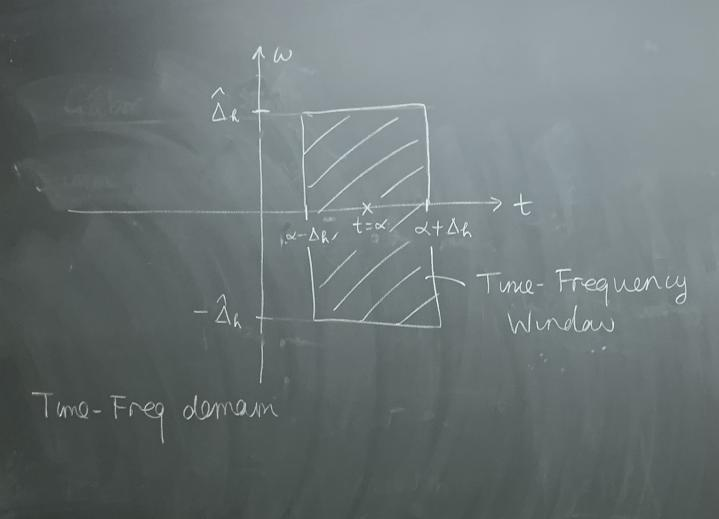
\includegraphics[width=0.5\textwidth]{Figures/lec6-1.png}\]
This is called the Time-Frequency Window on $(\alpha - \Delta_h, \alpha + \Delta_h) \times (-\widehat{\Delta}_h, \widehat{\Delta}_h)$. In other words, filtering gives information about $f(t)$ and $\widehat{f}(\omega)$ over a time-frequency window.\\

We note that the area of this window is bounded by
\[(2 \Delta_h)(2 \widehat{\Delta}_h) \geq 2\]

We have two significant issues:
\begin{itemize}
    \item The area of the time-frequency window is limited
    \item We have flexibility to shift the time-window by varying $\alpha$, but there's no flexibility to vary the frequency as it is always centered on $\omega = 0$.
\end{itemize}

\begin{question}
    Can we try to limit the area of the time-frequency window?
\end{question}

\begin{example}
    Here are some possible attempts:
    \begin{enumerate}
        \item Try $h(t) = \begin{cases} 
        \frac{1}{2\epsilon},\ |t| \leq \epsilon\\
        0,\ \text{otherwise}
        \end{cases}$, then $\widehat{h}(\omega) \sim \frac{\sin(\omega t)}{\omega t}$. Then we have that
        \begin{align*}
            \widehat{\Delta}_h &= \lim_{R \to \infty} \int_{-\infty}^\infty |\omega| |\widehat{f}(\omega)|^2 d\omega\\
            &= \infty
        \end{align*}
        So the radius is not good.
        \item Let's try the Gaussian filter $h(t) = e^{-t^2/2}$, then $\Delta_h \cdot \widehat{\Delta}_h = 1/2$. This suggests that a Gaussian filter should be optimal, but this function is globally supported. We do have rapid decay, and
        \[h(\alpha - t) = e^{-(t-\alpha)^2/2} \approx 0 \text{ when $|t - \alpha|$ is ``large"}\]
        In practice, we would just approximate using a Gaussian filter.
    \end{enumerate}
\end{example}

\begin{question}
    Can we try to move the time-frequency window vertically so that it can be centered on a given frequency $\xi$?
\end{question}

\begin{proof}[Answer]
    Yes! This is solved by what's known as the Gabor transform. Gabor actually won a Nobel Prize for discovering holograms. He was also a member of Fellows of the Royal Society.
\end{proof}

Now, let's consider
\[g(t) = (h * f)(t) \text{ or } \widehat{g}(\omega) = H(\omega) \widehat{f}(\omega)\]
given information around $\omega = 0$.

\begin{idea}
Let's try to shift the spectrum of $f$ before filtering!
\end{idea}

Recall we have that
\[f(s) =\frac{1}{2\pi} \int_{-\infty}^\infty e^{i\omega s} \widehat{f}(\omega) d\omega\]
This is a super-position of frequencies. Hence
\begin{align*}
    e^{-i\xi s} f(s) &= \frac{1}{2\pi} \int_{-\infty}^\infty e^{i(\omega - \xi)s} \widehat{f}(\omega) d\omega\\
    &= \frac{1}{2\pi} \int_{-\infty}^\infty e^{i\omega s} \widehat{f}(\omega + \xi) d\omega
\end{align*}
This shows that the spectrum of $f$ is shifted by an amount $\xi$ (sine $\widehat{f}(\omega) \to \widehat{f}(\omega + \xi)$).\\

\begin{definition}
Applying the filter to the resulting function gives the \textbf{Gabor transform}:
\[G_h(\alpha, \xi) \coloneqq (h* e^{-i\xi s}f(s))(\alpha) = \int_{-\infty}^\infty e^{-i\xi s} f(s) h(\alpha - s) ds\]
\end{definition}

In the time-frequency window, we now have
\[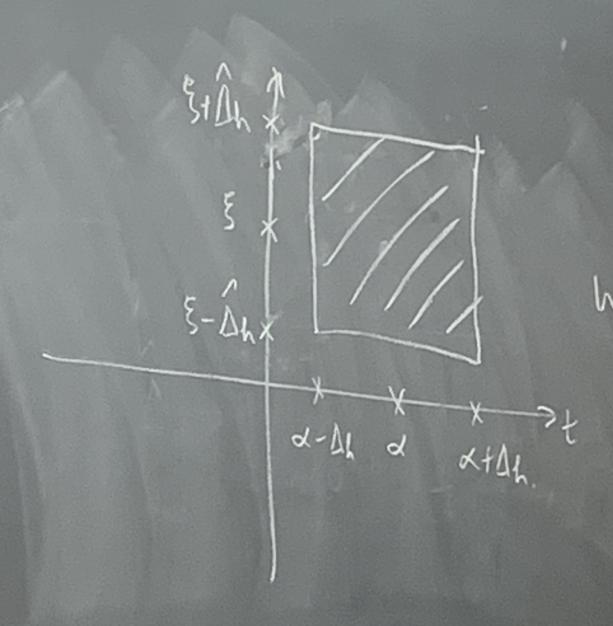
\includegraphics[width=0.5\textwidth]{Figures/lec6-2.png}\]

This is also a special case of what's known as a ``short time Fourier transform".

\newpage
\section{Lecture 7 - 2/8/2023}

Recall last lecture - given a special filter $\{h(t)\ :\ t \in \Rbb\}$, then we define the Gabor transform as
\[(G_h f)(\alpha, \xi) = \int_{-\infty}^\infty ds f(s) e^{-i\xi s} h(\alpha - s)\]
The idea is that - by varying $\alpha$ and $\xi$, we can shift the window horizontally and vertically across the time-frequency domain, around spatial location $\alpha$ and frequency $\xi$.

\begin{proposition}
    The Gabor transform gives a time-frequency window
    \[(\alpha - \Delta_h, \alpha + \Delta_h) \times (\xi - \widehat{\Delta}_h, \xi + \widehat{\Delta}_h)\]
    ie. window has area
    \[2 \Delta_h 2 \widehat{\Delta}_h \geq \frac{2 \cdot 2}{2} = 2\]
\end{proposition}

\begin{proof}
    We note that $h(\alpha - s)$ is centered on $\alpha$ with spread being $\Delta_h$ and $e^{-i\xi s}$ has no contribution to the time domain, thus clearly the temporal window is given by $(\alpha - \Delta_h, \alpha + \Delta_h)$.\\\\
    By Parserval's Identity, we note that
    \[(G_h f)(\alpha, \xi) = \frac{1}{2\pi} \int_{-\infty}^\infty d\omega \widehat{f}(\omega) \overline{?}\]
    where the term under the complex conjugation is exactly the Fourier transform of $e^{+i \omega s} h(\alpha - s)$, which is
    \begin{align*}
        \int_{-\infty}^\infty e^{-i\omega s} e^{i \xi s} h(\alpha - s) ds &= \int_{-\infty}^\infty e^{-i(\omefa - \xi)s} h(\alpha - s) ds\\
        &= \int_{-\infty}^\infty e^{-i(\omega - \xi)\alpha} e^{i(\omega - \xi)t} h(t) dt \tag*{Let $t = \alpha - s$}\\
        &= e^{-i(\omega - \xi)\alpha} int_{-\infty}^\infty e^{-i(\xi - \omega)t} h(t) dt\\
        &= e^{-i(\omega - \xi)\alpha} \widehat{h}(\xi - \omega)
    \end{align*}
    Thus, we have that
        \[(G_h f)(\alpha, \xi) = \frac{1}{2\pi} \int_{-\infty}^\infty d\omega \widehat{f}(\omega) e^{+i(\omega - \xi)\alpha} \overline{\widehat{h}(\xi - \omega)}\]
        Hence, we have centering on $\omega = \xi$ on the frequency domain and width of window $\widehat{\Delta}_h$.
\end{proof}

\begin{example}
    Consider a signal $\{f(t) = 1\ :\ t\in \Rbb\}$ and $h(t) = e^{-t^2/2}$, then
    \begin{align*}
        (G_h f)(\alpha, \xi) &= \int_{-\infty}^\infty dt f(t) e^{-i\xi t} e^{-(t-\alpha)^2/2}\\
        &= e^{-i\xi \alpha} \int_{-\infty}^\infty e^{-(t-\alpha)^2/2 - i \xi t}\\
        &\sim e^{-i\xi \alpha} e^{-\xi^2/2}
    \end{align*}
    In particular, we note that $|G_h f| = e^{-\xi^2/2}$ with the graph:
    \[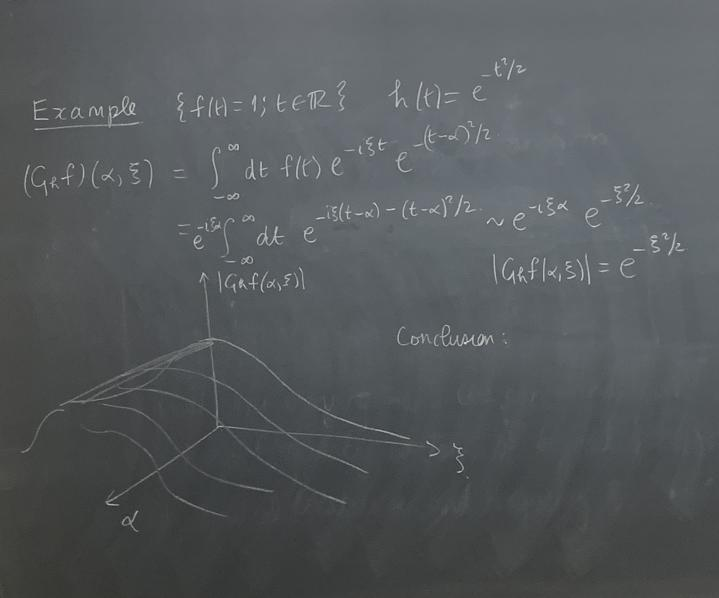
\includegraphics[width=0.5\textwidth]{Figures/lec7-1.png}\]
    Just analyzing the graph, we see that $|G_h f|$ is not varying in intensity in time, so there's no spatial localization at all. $|G_h f|$ is largest when $\xi = 0$, so the largest frequency content of the signal is around where $\xi = 0$, hence the dominant frequency is $\xi = 0$.
\end{example}

\begin{question}
    How to compute/approximate $G_h f$ when $f$ is not so simple?
\end{question}

We always make $h(t) = e^{-t^2/2}$ as our filter, to compute a numerical approximation, here are a few issues:
\begin{enumerate}
    \item $f(t)$ may be given only partially, e.g. only at certain points or on a limited range. Suppose we have $\{f(t): -w < t < w\}$ for some $w$. So the first approximation we need is
    \[(G_h f)(\alpha, \xi) \approx \int_{-w}^w dt f(t) e^{-i\omega t} e^{-(t- \alpha)^2/2}\]
    This is a good approximation if $f(t)$ decays rapidly outside. We also expect this to be a good approximation even if $f$ does not decay, provided that $\alpha$ is located ``well-inside" $(-w, w)$.
    \item We still can't compute analytically. Let's try to use the Trapezoidal Rule with nodes indexed by $-N, -N+1,..., 0, ..., N$ (choose $N$ large enough), then
    \[\approx \frac{W}{N} \sum_{m = -N}^N '' e^{-i \xi t_m} e^{-(t_m - \alpha)^2/2} f(t_m)\]
    where $t_m = m W/N$ for $m = -N, ..., N$ (the $\sum''$ means the first and the last term are halved).
    \item This could be very expensive if $N >> 1$ and/or $W >> 1$, we note that
    \[e^{-t^2/2} < 10^{-6} \text{ when } |t| > 5.6\]
    Therefore we are only going to sum over $N$ such that $|t_m - \alpha| < 6$, ie. only when
    \[-6N/W < m - \frac{N\alpha}{W} < 6N/W\]
    Hence combining our approximations gives
    \[(G_h f)(\alpha, \xi) \approx \frac{W}{N} \sum_{m = Lo}^{m = Hi}  e^{-i \xi t_m} e^{-(t_m - \alpha)^2/2} f(t_m)\]
    where
    \[Lo \coloneqq \max(-N, \lfloor frac{N}{W}(\alpha - 6) \rfloor)\]
    \[Hi = \min(N, \lceil N/W(\alpha + 6) \rceil)\]
    \[t_m = mW/N\]
    % \mattie{Fix this later }
\end{enumerate}

\newpage
\section{Lecture 8 - 2/10/2023}

\subsection{Gabor Transform (Continued)}
We recall that the Gabor transform was defined
\[(G_h f)(\alpha, \xi) = \int_{-\infty}^\infty f(t) e^{-i\xi t} e^{-(t- \alpha)^2/2} dt\]

The Gabor Transform enable us to do time-frequency analysis. In particular we can plot the following \textbf{spectrogram} and center on some window $(\alpha, \xi)$ with width $2\Delta_h$ and height $2 \widehat{\Delta}_h$:
\[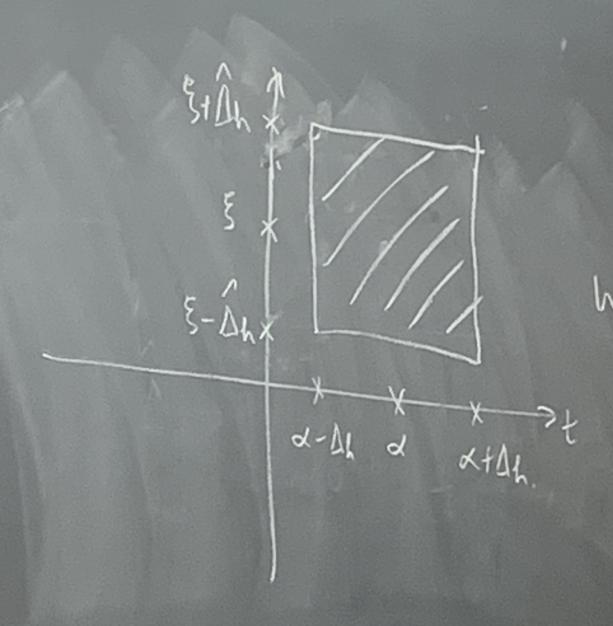
\includegraphics[width=0.5\textwidth]{Figures/lec6-2}\]
But since we have this fundamental restriction on the area of the window,
$(G_h f)(\alpha, \xi) \sim $ average of $f$ and $\hat{f}$ over the window.\\\\

\begin{example}
   We can't concentrate this around points because of the fundamental limit on the area of the window, hence the spectrogram has some imperfections going on:
       \[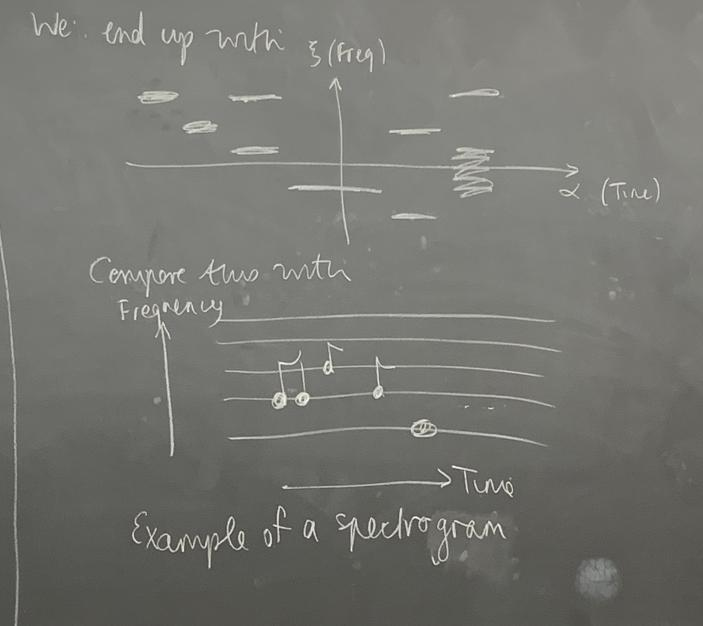
\includegraphics[width=0.3\textwidth]{Figures/lec8-1}\]
   We can compare this with a music sheet. In particular, a music sheet is really an example of a spectrogram and is in fact a perfect spectrogram, as you know exactly what frequencies should occur at each time.
\end{example}

Unfortunately, Gabor transform is limited by the time-frequency uncertainty principle, but we can change the aspect ratio of the time-frequency window to focus on localization in either time or frequency.\\

To decrease $\Delta_h$, we want to decay our $e^{-t^2/2}$ faster, to do this we can consider $e^{-\epsilon t^2/2}$. If we choose $\epsilon > 1$, we tighten the time window. If $\epsilon < 1$, we tighten the frequency window.\\

A discontinuity at time $t$ corresponds to the existence of all frequencies around time $t$.

\begin{claim}
Varying $\epsilon$ is more useful than varying $\xi$ and/or $\alpha$.
\end{claim}

\begin{question}
    Why don't we try to sacrifice a parameter?
\end{question}

\subsection{Varying $t-\omega$ Aspect Ratio Transform}

Let $\{h(t): t \in \Rbb\}$ be a given filter and define a new transform
\[W_h(\alpha, a) = \int_{-\infty}^\infty f(t) h(\frac{\alpha - t}{a}) dt\]
By varging 'a', we can change the aspect ratio of the window (we are not normalizing yet)
\[\Delta_h^2 \sim \int_{-\infty}^\infty (t - t^*) |h(t)|^2 dt\ \ (a = 1)\]
\[\Delta_{h, a}^2 \sim \int_{-\infty}^\infty (t - t^*)^2 |h(t/a)|^2 dt\]

Without loss of generality, let's say $t^* = 0$, then
\begin{align*}
    \Delta_{h, a}^2 &\sim \int_{-\infty}^\infty t^2 |h(t/a)|^2 dt\\
    &=a^3 \int_{-\infty}^\infty (t/a)^2 |h(t/a)|^2 d(t/a)\\
    &= a^3 \int_{-\infty}^\infty s^2 |h(s)|^2 ds
\end{align*}
Recall we also have to normalize this, and
\[||h(t/a)||^2 = a \int_{-\infty}^\infty |h(t/a)|^2 \frac{dt}{a} = a ||h||^2\]
Hence, we have that
\[\Delta_{h, a}^2 \sim a^2 \Delta_h^2\]

Let's try to rescale $h$ so that $h(\frac{\bullet}{a})$ is independent of $|a|$, ie. let's define
\[h_a(t) = \frac{1}{\sqrt{a}} h(t/a)\]
Hence we note that
\[||h_a(t)||^2 = \frac{1}{a} \int_{-\infty}^\infty |h(t/a)|^2 dt = \int_{-\infty}^\infty |h(s)|^2 ds\]
This value is now independent of $a$!\\\\

We now arrive at a new type of transform
\[(W_h f)(\alpha, a) = \frac{1}{\sqrt{a}} \int_{-\infty}^\infty f(t) h(\frac{\alpha - t}{a}) dt\]

This is also called the \textbf{continuous Wavelet transform}. In particular, $h$ is the \textbf{analyzing wavelet}! We want to choose $h$ so that it doesn't pick up any DC components, namely that
\[\int_{-\infty}^\infty h(s) ds = 0\]
For covenience, we also want $h(s)$ to be compactly supported. So we want something like:
\[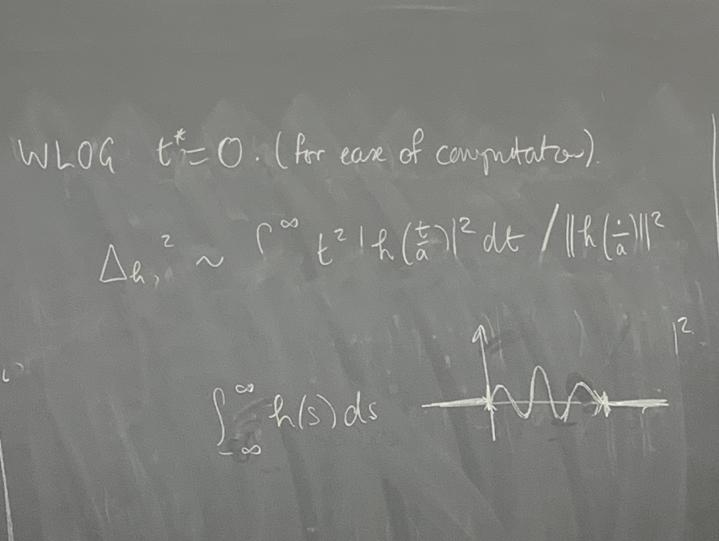
\includegraphics[width=0.5\textwidth]{Figures/lec8-2}\]
Which looks like the shape of a wavelet!

\newpage
\section{Lecture 9 - 2/13/2023}

\subsection{Continuous Wavelet Transform}
At the end of the last class, we claim up with the following
\begin{definition}
    Let $\psi$ be a real-valued function with $\psi(t)$, $|t|^{1/2} \psi(t)$, and $t \psi(t)$ all integrable with finite energy (ie. square integrable), and that $\widehat{\psi}(0) = 0$ (note this is true if and only if $\int_{-\infty}^\infty \psi(t) dt = 0$). Then the \textbf{continuous wavelet transform (CWT)} of a signal $f(t)$ is
    \[(W_\psi f)(\alpha, a) = \frac{1}{\sqrt{a}} \int_{-\infty}^\infty f(t) \psi(\frac{\alpha - t}{a}) dt,\ \alpha \in \Rbb, a > 0\]
    The landpass filter $\psi$ is called the ``analyzing wavelet".
\end{definition}

\begin{question}
    What are the Time-Frequency properties of this?
\end{question}

In the time domain, we get a window around $t = \alpha$ and radius is given by
\begin{align*}
    \Delta_\psi^2 &= \int_{-\infty}^\infty t^2 \psi(\frac{\alpha - t}{a})^2 dt / \int_{-\infty}^\infty \psi(\frac{\alpha - t}{a})^2 dt\\
    &= a^2 \int_{-\infty}^\infty s^2 \psi(s)^2 ds / \int_{-\infty}^\infty \psi(s)^2 ds \tag*{Let $s = (\alpha - t)/a$}\\
    &= (a \Delta_\psi)^2
\end{align*}
So the time window is $(\alpha - a \Delta_\psi, \alpha + a \Delta_\psi)$.\\

In the frequency domain, we use Parserval's Identity to write $W_\psi f$ in terms of $\widehat{f}(\omega)$. To do this, we need the Fourier Transform of $t \mapsto \psi(\frac{\alpha - t}{a})$. Using techniques in Homework $1$, we get
\[\int_{-\infty}^\infty e^{-i\omega t} \psi(\frac{\alpha - t}{a}) dt = a e^{-i\omega \alpha} \overline{\widehat{\psi}(a\omega)}\]

Hence, by Parserval's Identity, we have that
\[(W_\psi f)(\alpha, a) = \frac{\sqrt{a}}{2\pi} \int_{-\infty}^\infty \widehat{f}(\omega) e^{i \omega \alpha} \widehat{\psi}(a\omega) d\omega \]
This shows that the frequency window is centered on $\omega = 0$ and has radius, with a very similar calculation as before
\begin{align*}
    \widehat{\Delta}^2_{\psi, a} &= \frac{1}{a^2} \widehat{\Delta}_\psi^2
\end{align*}
Hence we have the frequency window on $(-\frac{1}{a} \widehat{\Delta}_\psi^2, + \frac{1}{a} \widehat{\Delta}_\psi^2)$.\\

Our time frequency window looks like:
\[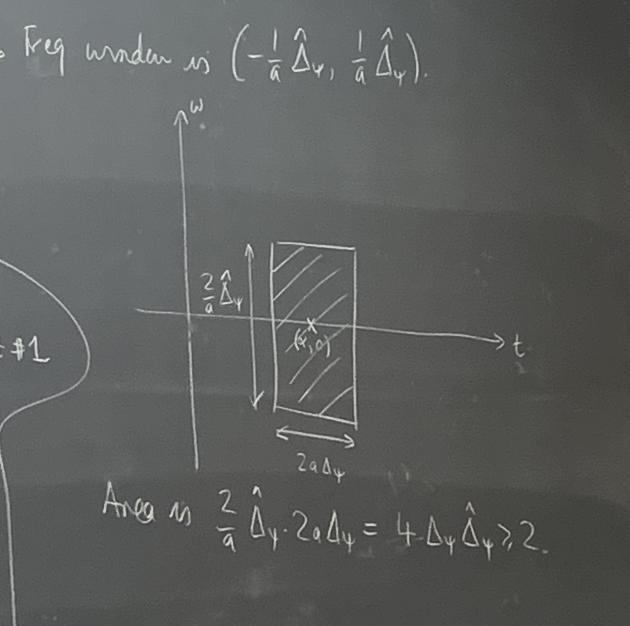
\includegraphics[width=0.5\textwidth]{Figures/lec9-p1.png}\]
with area being $\frac{2}{a} \Delta_\psi (2a \widehat{\Delta}_\psi) = 4 \Delta_\psi \widehat{\Delta}_\psi \geq 2$. We didn't change the area of the window, but we can change the aspect ratio by varying the value of $a$.\\

The flexibility to vary $a$ allows us to change the scale at which resolve time and/or frequency. In a sense, $a$ is similar to a ``zoom factor" on a microscope that allows us to focus in a local feature.

\begin{definition}
    A band-pass filter $\psi(t)$ is a filter with dc component being $0$, ie $\int_{-\infty}^\infty \psi(t) dt = 0$
\end{definition}

\begin{example}
    The Haar Wavelet is
\[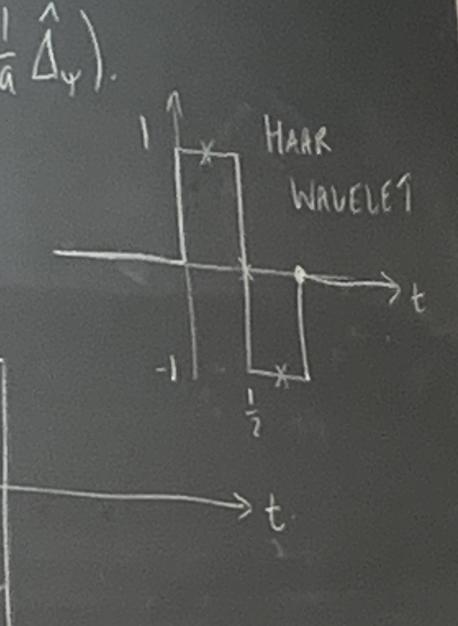
\includegraphics[width=0.3\textwidth]{Figures/lec9-p2.png}\]
    This is in some sense the simplest wavelet. It is locally supported, band-pass, etc.
\end{example}


\subsection{Smoothness of Functions}
 The actual value of the filter function doesn't matter, what we care about more is how the function varies over time! This concerns with the ``smoothness" of a given function $f$, ie. we want to know where it is not smooth.

 \begin{question}
     How do we measure smoothness?
 \end{question}

\begin{definition}
    We say $f$ is Lipschitz-continuous at $s$ with exponent $\mu$ if there exists $K < \infty$ and $\mu \in (0, 1)$
    \[|f(s) - f(t)| \leq K |s - t|^\mu \]
    , for $t$ close to $s$. The idea here is that the larger $\mu$ is, the more ``differentiable" the function is.
\end{definition}

\begin{question}
    Can we figure out $s$ and $\mu$ by looking at $\widehat{f}(\omega)$ is?
\end{question}

\begin{theorem}
    If $\widehat{f}$ satisfies $\int_{-\infty}^\infty |\widehat{f}(\omega)| (1 + |\omega|^\mu) d\omega < \infty$, then $f$ is Lipschitz continuous every where with exponent $\mu$.
\end{theorem}

\begin{proof}
    Let's consider $\frac{|f(s) - f(t)|}{|s - t|^\mu}$ and figure out how large $\mu$ can be, so
    \begin{align*}
        f(s) &= \frac{1}{2\pi} \int_{-\infty}^\infty \widehat{f(\omega)} e^{+i\omega s} d\omega\\
        f(t) &= \frac{1}{2\pi} \int_{-\infty}^\infty \widehat{f(\omega)} e^{+i\omega t} d\omega\\
        f(s) - f(t) &= \frac{1}{2\pi} \int_{-\infty}^\infty \widehat{f}(\omega) (e^{i\omega s} - e^{i\omega t}) d\omega
    \end{align*}
    We observe that
    \begin{align*}
        |e^{i\omega s} - e^{i \omega t}| &\leq 2 \tag*{By Triangle's Inequality, this is best bound when $\omega >> 0$} 
    \end{align*}
    On the other hand, we have that
    \begin{align*}
        |e^{i\omega s} - e^{i \omega t}|  &= |[e^{i \omega \theta}_t^s]|\\
        &= |\int_{t}^s i \omega e^{i \omega \theta} d\theta|\\
        &\leq |\int_t^s d\theta |\omega||\\
        &\leq |\omega| \cdot |s - t| \tag*{Good when $s$ is close to $t$ and $\omega$ is small}
    \end{align*}
    Now, we have that
    \[        \frac{|e^{i\omega s} - e^{i \omega t}|}{|s - t|^\mu} \leq \begin{cases}
            2|s - t|^{-\mu},\\
            |\omega| |s - t|^{1-\mu}
        \end{cases}\]
    If $|s - t| > |\omega|^{-1}$, then $|s - t|^{-1} < |\omega|$, hence $|s - t|^{-\mu} < |\omega|^\mu$.\\\\
    If $|s - t| < |\omega|^{-1}$, then $|s - t|^{1- \mu} < |\omega|^{\mu - 1}$, hence $|\omega| |s - t|^{1-\mu} < |\omega|^\mu$, thus we always have that
    \[ \frac{|e^{i\omega s} - e^{i \omega t}|}{|s - t|^\mu} \leq  C |\omega|^\mu\]
    for some constant $C$, hence we have that
    \begin{align*}
    \frac{|f(s) - f(t)|}{|s - t|^\mu} &\leq \frac{1}{2\pi} \int_{-\infty}^\infty |\widehat{f}(\omega)| \cdot \frac{|e^{i\omega s} - e^{i\omega t}|}{|s - t|^\mu} d\omega\\
    &\leq \frac{C}{2\pi} \int_{-\infty}^\infty |\widehat{f}(\omega)| (1 + |\omega|^\mu) d\omega\\
    &< \infty
    \end{align*}
\end{proof}

Good news - looking at the decay of $|\widehat{f}(\omega)|$ as $|\omega| \to \infty$ tells us about the smoothness of $f$.\\\\

Bad news - this tells us nothing about the local smoothness, ie. how doe sthe smooth vary with respect to position! ($\mu$ is the lower bound on the smoothness of all the points).\\\\

Recall that for $t \mapsto f(t - \alpha)$, the Fourier transform is $\omega \mapsto e^{i \alpha \omega} \widehat{f}(\omega)$, but the fourier transform DOES NOT translate anything, so its modulus is the same as $|\widehat{f}(\omega)|$. Hence no matter how we try to tweak around the theorem, we won't have the local information.

\newpage
\section{Lecture 10 - 2/15/2023}

Recall that we have established, last time, that:
\begin{itemize}
    \item Locally Lipschitz - $f$ is locally Lipschistz at $\alpha$ with exponent $\mu$ if
    \[|f(\alpha) - f(t)| \leq K|\alpha - t|^\mu\]
    where $\mu$ indicates/measures how smooth $f$ is at $\alpha$
    \item Can we deduce $\mu$ without looking directly at $f(t)$ and $t \in \Rbb$
    \item We proved last lecture that:
\begin{theorem}
    If $\widehat{f}$ satisfies
    \[\int_{-\infty}^\infty |\widehat{f}(\omega)| (1 + |\omega|^\mu) d\omega < \infty\]
    then $f$ is globally Lipschitz with exponent $\mu$.
\end{theorem}
    \item As a corollary, $f(t) = \frac{1}{2\pi} \int_{-\infty}^\infty e^{i\omega t} \widehat{f}(\omega) d\omega$ implies that
    \[|f(t)| \leq \frac{1}{2\pi} \int_{-\infty}^\infty |\widehat{f}(\omega)| d\omega < \infty\]
    So the $1 +$``something" means $f$ is a well-defined behavior. However, this theorem only tells us the \textbf{global $\mu$}, but some parts of $f$ might do better than this global $\mu$. This means we have to analyze the behaviors of $f$ more locally.
\end{itemize}

\begin{question}
    Can we find a better way to identify $\mu$ and hopefully how smooth this is at $\alpha$?
\end{question}

Consider the Lipschitz condition, 
\[|f(\alpha) - f(t)| \leq K |\alpha - t|^\mu\]
Let's write $t = \alpha - as$ for some $a > 0$ and $s$, then we have that
\[|f(\alpha) - f(\alpha - as)| \leq K a^\mu |s|^\mu\]
Suppose we scale $a \mapsto a/2$, then the $K a^\mu |s|^\mu$ becomes $K a^\mu |s|^\mu/2^\mu$. This means that we can interpret Lipschitz as a scaling relation where $\mu$ measures the relative change on $f$ when the arguments get closer (recall $0 < \mu < 1$).\\

This suggests that by varying ``$a$", we should be able to detect the value of $\mu$ when we examine the change in $f$.\\

Let's recall the continuous wavelet transform:
\[(W_h f)(\alpha, a) = \frac{1}{\sqrt{a}} \int_{-\infty}^\infty f(t) h(\frac{\alpha - t}{a}) dt\]
We can interpret $a$ as a ``zoom" or ``scale" factor, and $W_h f$ is the response to the scaling. We claim it is plausible that we can use the CWT to identity $\mu$!\\

We will now make this assertion more precise:
\begin{align*}
    (W_h f)(\alpha, a) &= \frac{1}{\sqrt{a}} \int_{-\infty}^\infty f(s) h(\frac{\alpha - s}{a}) ds\\
    &= \sqrt{a} \int_{-\infty}^\infty f(\alpha - at) h(t) dt \tag*{Let $t = \frac{\alpha - s}{a}$}
\end{align*}
When we change $a \mapsto a/2$, is there a $\mu$-dependent response above? There's no apparent behavior that depends on $\mu$, the scalar doesn't matter, $f(\alpha - at)$ converges to $f(\alpha)$, but this has nothing to do with $\mu$.\\

But, we recall in the Lipschitz condition, we are really comparing $|f(\alpha) - f(\alpha - at)|$, can we introduce a $f(\alpha)$ in here? Indeed, let we assume that $\int_{-\infty}^\infty h(t) dt = 0$, then
\[(W_h f)(\alpha, a) = \sqrt{a} \int_{-\infty}^\infty [f(\alpha - at) - f(\alpha) + f(\alpha)] h(t) dt = \sqrt{a} \int_{-\infty}^\infty [f(\alpha - at) - f(\alpha)] h(t) dt + 0  \]

Estimate using Lipschitz, 
\begin{align*}
    |W_h f(\alpha, a)| &\leq \sqrt{a} \int_{-\infty}^\infty |f(\alpha - at) - f(\alpha)| |h(t)| dt\\
    &\leq \sqrt{a} \int_{-\infty}^\infty K|at|^\mu |h(t)|\ dt \tag*{Lipschitz Continuity}\\
    &= a^{1/2 + \mu} K \int_{-\infty}^\infty |t|^\mu |h(t)|\ dt
\end{align*}
This suggests that we can detect $\mu$ locally by seeing how the Wavelet transform behaves with ``$a$"!

\begin{example}
    Consider the function $f(t) = |t|$, this is not smooth at $t = 0$. We see that
    \[|f(t) - f(s)| = ||t| - |s|| \leq |t - s|^\mu\]
    The highest value of $\mu$ should be $1$! Because this is just the reverse triangle inequality. Let's consider
    \begin{enumerate}
        \item $h(t) = e^{-t^2/2}$, then
        \begin{align*}
            (W_h f)(0, a) &= \sqrt{a} \int_{-\infty}^\infty |\alpha - at| e^{-t^2/2} dt
        \end{align*}
        There's no $\mu$-dependent response here... This is no good because $h(t)$ is not an analyzing wavelet! ($\int_{-\infty}^\infty h(t) dt \neq 0$)
        \item Let $h(t)$ be the Haar wavelet:
        \[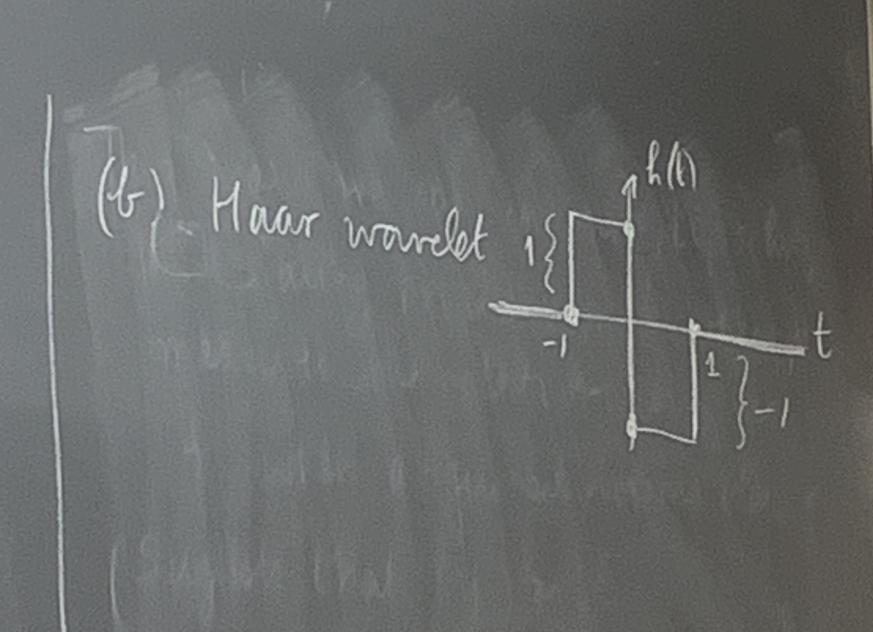
\includegraphics[width=0.3\textwidth]{Figures/lec10-p1.png}\]
        and we have that
        \begin{align*}
            (W_h f)(0, a) &= \sqrt{a} \int_{-\infty}^\infty h(t) |at| dt\\
            &= a^{3/2} \int_{-\infty}^\infty |t| h(t) dt
        \end{align*}
        This varies as $a^{3/2} = a^{1/2 + 1}$, BUT $\int_{-\infty}^\infty |t| h(t) dt = 0$, so this actually doesn't change as you change $a$. Hence this is not very useful. But we can still look at $(W_h f)(\alpha, a)$ with $\alpha \approx 0$.
        \item Derivative Gaussian Wavelet - this is $h(t) = - \frac{d}{dt} e^{-t^2/2} = t e^{-t^2/2}$, which graphically:
        \[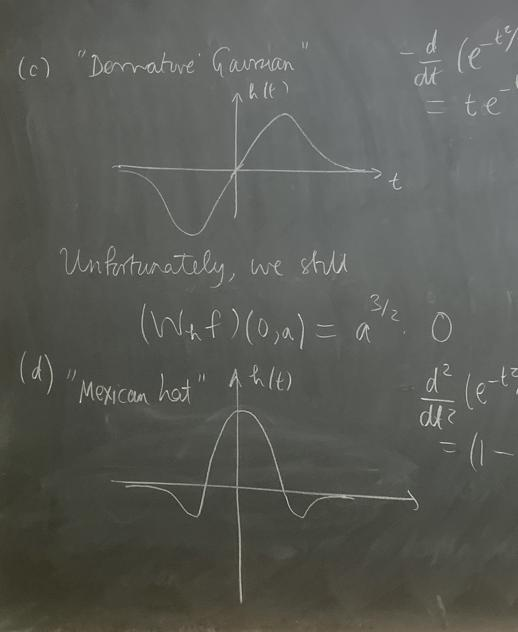
\includegraphics[width=0.3\textwidth]{Figures/lec10-p2.png}\]
        Unfortunately, this has the same problem as
        \[(W_h f)(0, a) = a^{3/2} \cdot 0 = 0\]
        \item Let's consider $h(t) = \frac{d^2}{dt^2}(e^{-t^2/2}) = (1 - t^2) e^{-t^2/2}$, this is called the ``Mexican Hat Wavelet", whose picture is given above.
        We have that
        \[(W_h f)(0, a) = \sqrt{a} \int_{-\infty}^\infty |t| h(t) dt = -2 a^{3/2}\]
        THis does respond to $a^{1/2 + \mu}$! We also observe that
        \[(W_h f)(\alpha, a) = -2 a^{3/2} e^{-\alpha^2/(2a^2)}\]
        Plotting $\alpha$ against $a > 0$, recall that $e^{-\alpha^2 /2a^2} \approx 0$ when $|\alpha/\sqrt{2a}| \geq 6$
        \[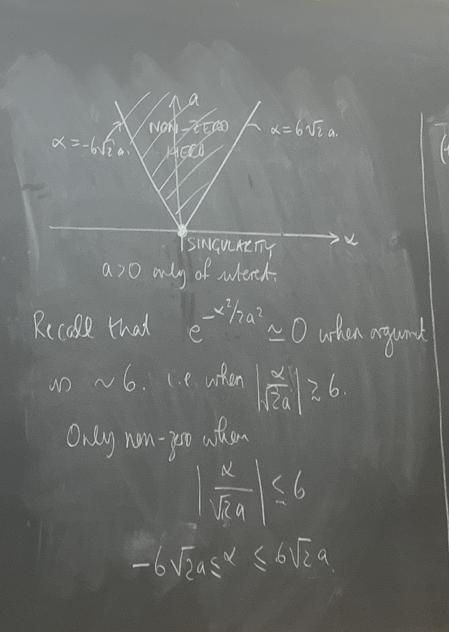
\includegraphics[width=0.3\textwidth]{Figures/lec10-p4.png}\]
        This points to where the singularity is, the rate of increase around the singularity is how bad the singularity is.
    \end{enumerate}
\end{example}

\newpage
\section{Lecture 11 - 2/17/2023}

\subsection{Higher Moments}
We recall that last lecture, we obtained the following two equivalent formulation of the Continuous Wavelet Transform:
\begin{align*}
    (W_h f)(\alpha, a) &= \frac{1}{\sqrt{a}} \int_{-\infty}^\infty f(t) h(\frac{\alpha - t}{a}) dt\\
    &= \sqrt{a} \int_{-\infty}^\infty f(\alpha - as) h(s) dt \tag*{Let $s = \frac{\alpha - t}{a}$}
\end{align*}

\begin{question}
    What key property of the Mexican hat makes it a better filter for $f(s) = |s|$?
\end{question}

Indeed, let $h(t) = (1 - t^2) e^{-t^2/2}$, we first note 
\[\widehat{h}(0) = \int_{-\infty}^\infty h(s) ds = 0\]
Thus, we have that
\begin{align*}
    (W_h f)(\alpha, s) &= \sqrt{a} \int_{-\infty}^\infty f(\alpha - as) h(s) ds\\
    &= \sqrt{a} \int_{-\infty}^\infty [f(\alpha - as) - f(\alpha)] h(s) ds
\end{align*}
This allows us to use the Lipschitz property!

\begin{question}
    Can we look at higher degrees of smoothness? (ie. when the derivatives are also smooth)
\end{question}

Indeed, we can think of the condition $\int_{-\infty}^\infty h(s) ds = 0$ as the fact that the zeroth moment of $h(s)$ is $0$. If $h(s)$ vanishes on higher moments too, we can write
\[(W_h f)(\alpha, a) = \sqrt{a} \int_{-\infty}^\infty [f(a - \alpha s) - \text{linear polynomial}] h(s) ds\]

What is the term $f(a - \alpha s) - \text{linear polynomial}$? Well, we can write 
\[f(s) = f(0) + s f'(0) + ...\]
using Taylor expansions. For the zero-th moment, we have that
\[f(s) - f(0) = s f'(0) + ... \]
In this case, we have filtered out the constant term (ie. the DC component). For higher order moments, we want to filter out more terms. To do this, we want the first $n$ orders of $h(s)$ to be $0$, that is
\[\int_{-\infty}^\infty s^k h(s) ds = 0, 0 \leq k \leq n\]

\begin{example}
    If we look back at the Mexican Hat example again, we observe that
    \[\int_{-\infty}^\infty s (1 - s^2) e^{-s^2/2} ds = 0\]
    Hence, the first order moment of the filter is also $0$.\\\\
    This means that $(W_h f)(\alpha, a) \approx 0$ at non-zero values too!\\\\
    If we recall the examples we used last time, the Gaussian filter $h(t) = e^{-t^2/2}$ fails because its zeroth moment is non-zero. The Haar wavelet fails because its first moment is non-zero, hence it is sensitive to derivatives. The first moment of the derivative Gaussian is similarly also non-zero.
\end{example}

\subsection{Criterion for Selecting a Wavelet}

In general we want out filter $h(s)$ to satisfy:
\begin{itemize}
    \item $\int_{-\infty}^\infty s^m h(s) ds = 0$ for $m = 0, 1, ..., M$ where $M$ is taken to be necessary. This implies that $h(s)$ should also be oscillating.
    \item $h(s)$ has rapid decay or compactly supported.
\end{itemize}

Note that sometimes we do not want to make $M$ too big. For example,
\[\frac{d^{1066}}{d t^{1066}} (e^{-t^2/2})\]
is a good filter moment wise, but it is really complicated to work with because we will be dealing with $e^{-t^2/2} \times \text{polynomial of degree $1066$}$.

Thus, we have that
\[(W_h f)(\alpha, a) = \frac{1}{\sqrt{a}} \int_{-\infty}^\infty f(t) h(\frac{t - \alpha}{a}) dt\]
Generally, this integral is not directly solvable, so we would want to obtain a numerical approximation, for fixed $\alpha, a$, we have
\[(W_h f)(\alpha, a) \approx \frac{1}{\sqrt{a}} \sum_{n \in \Zbb} f(n) h(\frac{n - \alpha}{a})\]
where $f(n)$ is thought of as the ``digital representation" of $f$. This is because computers can't represent functions analytically, so we instead take at each digit.

\begin{definition}
    Let $\{f(t): t \in \Rbb\}$ be a signal, we call
    \[\{f(n): n \in \Zbb\}\]
    the digital representation of the signal.
\end{definition}

\newpage

\section{Lecture 12 - 2/19/2023}

\subsection{Band-Limited Signals and Shannon Sampling Theorem}

Consider the following problem:

\begin{question}
We have a digital phone exchange where calls are transmitted as digital signals. $\{f(t): t \in \Rbb\}$ is thought of as an analog signal, no information is really lost here, but now we only have packets of the signal (thought of as digital), so we only know the signal at integer values. In other words, we only have the information $\{f(m): m \in \Zbb\}$.\\

The question is - how often do we need to sample the signal in order to get a perfect reconstruction at the other end? (... why can we even consider getting a perfect reconstruction? If there's no constraint on the function other than continuity, you can find infinity many functions fitting through the digital signal.) 
\end{question}

At a mathematical level, the question makes no sense (because frequency can be arbitrarily high). However, in practice, we do have a constraint on the signal because we are thinking about this in the context of a ``phone exchange", so we are only interested in certain frequency ranges. It is then natural to consider signals such that the frequency is limited:
\[\widehat{f}(\omega) = 0 \text{ if $|\omega| > \Omega$}\]
for some $\Omega \geq 0$.\\

Let's now reformulate our question:
\begin{question}[Shannon's Problem]
    Suppose $f$ is band-limited by $\Omega$, how often do we need to sample $f$ in order to reconstruct $f$ from the digital samples?
\end{question}

\subsection{Poisson Summation Formula}
In order to answer this question, we derive a useful mathematical tool - the Poisson Summation Formula.\\

Suppose that $\widehat{f}(\omega)$ satisfies a decay condition (this holds for all band-limited signals but we are considering a more general case here):
\[|\widehat{f}(\omega)| \leq C (1 + |\omega|)^{-\alpha}\ \text{ for some $\alpha > 1$}\ (*)\]
(Note that the condition for Lipschitz $\alpha$ we proved implies this, but the converse is not true).\\\\

To see that band-limited signals satisfy this, we can choose $C = (1 + |\Omega|)^{\alpha} \cdot \max_{|\xi| \leq \Omega} |\widehat{f}(\xi)|$, hence
\[|\widehat{f}(\omega)| \leq \frac{(1 + |\Omega|)^{\alpha}}{(1 + |\omega|)^{\alpha}} \max_{|\xi| \leq \Omega} |\widehat{f}(\xi)|\]

In particular, $(*)$ means that
\[\int_{-\infty}^\infty |\widehat{f}(\omega)| d\omega \leq C \int_{-\infty}^\infty \frac{d\omega}{(1 + |\omega|)^\alpha} < \infty\]

Hence we have that
\[|\int_{-\infty}^\infty e^{i\omega t} \widehat{f}(\omega) d\omega| \leq \int_{-\infty}^\infty |\widehat{f}(\omega)| d\omega < \infty\]
Thus, \underline{Fourier series is well-defined and $f$ is well-defined}.\\

\begin{definition}
Let $p > 0$ be given, and define a periodisation of $\widehat{f}$ as follows:
\begin{align*}
    \widehat{f}_{per}(\omega) &= \sum_{k \in \Zbb} \widehat{f}(w + kp)
\end{align*}
Then, $\widehat{f}_{per}(\omega)$ is clearly periodic with period $p$. 
\end{definition}

\begin{proposition}
    $\widehat{f}_{per}(\omega)$ is well-defined for all $\omega \in \Rbb$.
\end{proposition}

\begin{proof}
    To see that the sum converges, we only need to consider $\widehat{f}_{per}(\omega)$ for $\omega \in [0, p]$ and note that
\begin{align*}
    \int_0^p |\widehat{f}_{per}(\omega)| d\omega &= \int_0^p |\sum_{k \in \Zbb} \widehat{f}(\omega + kp)| d\omega\\
    &\leq \sum_{k \in \Zbb} \int_0^p |\widehat{f}(\omega + kp)| d\omega\\
    &= \sum_{k \in \Zbb} \int_{kp}^{kp +p} |\widehat{f}(\xi)| d\xi \tag*{Let $\xi = \omega + kp$}\\
    &= \int_{-\infty}^\infty |\widehat{f}(\xi)| d\xi\\
    &< \infty
\end{align*}
\end{proof}

In particular, $\widehat{f}_{per}(\omega)$ has a discrete Fourier series.
\[\widehat{f}_{per}(\omega) = \sum_{n \in \Zbb} c_n e^{-2\pi i \omega n/p},\ \omega \in [0, p]\]
where
\[c_n = \int_0^p \frac{1}{p} \widehat{f}_{per}(\omega) e^{2\pi \omega n/p} d\omega\]
Computing $c_n$ explicitly:
\begin{align*}
    c_n &= \int_0^p \frac{1}{p} \widehat{f}_{per}(\omega) e^{2\pi \omega n/p} d\omega\\
    &= \frac{1}{p} \sum_{k \in \Zbb} \int_0^p \widehat{f}(\omega + kp) e^{2\pi i \omega n/p} d\omega\\
    &= \frac{1}{p} \sum_{k \in \Zbb} \int_{kp}^{kp+p} \widehat{f}(\xi) e^{2\pi i(\xi - kp)n/p} d\xi \tag*{Let $\xi = \omega + kp$}\\
    &= \frac{1}{p} \sum_{k \in \Zbb} \int_{kp}^{kp+p} \widehat{f}(\xi) e^{2\pi i(\xi)n/p}\cdot 1 d\xi\\
    &= \frac{1}{p} \sum_{k \in \Zbb} \int_{kp}^{kp+p} \widehat{f}(\xi) e^{2\pi i(\omega)n/p} d\omega\\
    &= \frac{1}{p} \int_{-\infty}^\infty \widehat{f}(\omega) e^{2\pi i \omega n/p} d\omega\\
    &= (\frac{2\pi}{p}) (\frac{1}{2\pi}) \int_{-\infty}^\infty \widehat{f}(\omega) e^{2\pi i \omega n/p} d\omega\\
    &= \frac{2\pi}{p} f(\frac{2\pi n}{p}) \tag*{By Fourier Inversion Formula}
\end{align*}

Hence, we obtain the Possion Summation Formula:
\begin{theorem}
Let $p > 0$ be fixed and $\widehat{f}$ be a function that satisfies then aforementioned decay condition, then
   $$\widehat{f}_{per}(\omega) = \frac{2\pi}{p} \sum_{n \in \Zbb} f(\frac{2\pi n}{p}) e^{-2\pi i \omega n/p}$$
for all $\omega \in [0, p]$
\end{theorem}

This is really useful for proving various identities:
\begin{corollary}[Basel Problem]
    $\sum_{n = 1}^\infty \frac{1}{n^2} = \frac{\pi^2}{6}$
\end{corollary}

\begin{proof}
    Exercise!
\end{proof}

\begin{remark}
    The closed form value of $\sum_{n = 1}^\infty \frac{1}{n^3}$ is not known! It's interesting to investigate why you can't use Possion Summation Formula to solve this.
\end{remark}

\end{document}
